% =====================================================================
%  석사학위논문 (한글)  --  이현주
%  CO2 전기환원(CO2RR)을 위한 경제적 고엔트로피 카바이드 전극촉매의
%  생성형 탐색 및 제일원리 검증
%
%  컴파일:  xelatex main_ko && xelatex main_ko   (목차/참조 위해 2회)
%  그림은 ../figures/ 에서 읽음 (CarbideMatterGen 파이프라인 산출물).
% =====================================================================
\documentclass[11pt,a4paper]{report}

\usepackage[margin=2.5cm]{geometry}
\usepackage{kotex}                 % 한글 (xelatex)
\usepackage{graphicx}
\graphicspath{{../figures/}}
\usepackage{amsmath,amssymb}
\usepackage{booktabs}
% --- siunitx 대체 경량 매크로 (패키지 의존성 회피) ---
\providecommand{\SI}[2]{#1\,#2}
\providecommand{\SIrange}[3]{#1--#2\,#3}
\providecommand{\angstrom}{\mbox{\AA}}
\usepackage{xcolor}
\usepackage{caption}
\usepackage[hidelinks]{hyperref}
\usepackage{enumitem}
\usepackage{tikz}
\usetikzlibrary{arrows.meta,positioning,fit,backgrounds,calc}
\emergencystretch=2em   % 한글+라틴 혼용 줄바꿈 overfull 완화

% \tbu: 실험 대기(빨강), \tbc: 진행 중 계산 대기(파랑)
\newcommand{\tbu}[1]{\textcolor{red!70!black}{\textbf{[#1 -- 실험 완료 후 업데이트 예정]}}}
\newcommand{\tbc}[1]{\textcolor{blue!60!black}{\textbf{[#1 -- 계산 완료 후 추가 예정]}}}
\newcommand{\dGCO}{\Delta G_{\mathrm{CO^*}}}
\newcommand{\dGH}{\Delta G_{\mathrm{H^*}}}
\newcommand{\dGCOOH}{\Delta G_{\mathrm{COOH^*}}}
\newcommand{\Ef}{E_\mathrm{F}}

\title{\bfseries CO\textsubscript{2} 전기환원(CO\textsubscript{2}RR)을 위한\\
경제적 고엔트로피 카바이드 전극촉매의\\
생성형 탐색 및 제일원리 검증\\[2pt]
\normalsize\mdseries --- CO 생성 활성점 설계에서 다중탄소 생성물까지}
\author{이현주 (Hyun-Ju Lee)\\[4pt]
\small 지도교수: [지도교수명]\\
\small [학과], [대학교]}
\date{2026년 6월}

\begin{document}
\maketitle

% =====================================================================
\chapter*{국문 초록}
\addcontentsline{toc}{chapter}{국문 초록}
이산화탄소 전기환원(CO\textsubscript{2}RR)은 재생 전력으로 CO\textsubscript{2}를 유용한 탄소
화합물---일산화탄소(CO)에서 에탄올과 같은 다중탄소(C\textsubscript{2+}) 연료까지---로 전환하여
인위적 탄소 순환을 닫는 핵심 경로이지만, 선택성이 높은 기존 촉매(Au, Ag 등)는 희소하고
고가이다. 이때 CO는 심화 환원 생성물로 가는 \emph{관문 중간체}이므로, 효율적 CO 생성과 경쟁하는
수소 발생(HER)의 억제는 모든 CO\textsubscript{2}RR 생성물의 공통 필요조건이다. 본 논문은
\emph{경제적인} CO\textsubscript{2}RR 카바이드 촉매를 고엔트로피 전이금속
카바이드(high-entropy carbide, HEC)의 화학 공간에서 직접 탐색하는 종단간(end-to-end)
\emph{생성형(generative)} 발견 파이프라인을 개발하고 적용한다. 물성 조건부 확산 모델
(미세조정된 \textsc{MatterGen})을 안정하고 금속성이며 일산화탄소를 방출하고 백금족 금속이
없는 조성으로 유도하며, 생성된 후보군을 조성 기반 대리지표, 기계학습 원자간 퍼텐셜(UMA)을
이용한 표면 자유에너지 스크리닝, 그리고 \textsc{Quantum ESPRESSO}에서의 밀도범함수이론(DFT)
검증의 깔때기를 통과시킨다. 하나의 파이프라인을 \emph{두 제약 집합}으로 구동하여, 우수한
전극촉매가 만족해야 할 네 설계 공리(활성·선택성·제조 가능성·경제성)가 생성 단계에서 어떻게
상호작용하는지를 통제 비교한다. \emph{캠페인 A}(활성-우선 기준선)는 6개의 백금족-무함유 HEC로
수렴하나, 이들은 금속열환원--\emph{산-침출} 합성의 필수 침출 단계에서 희토류가 용해되어 제조
불가이다 --- 제약 없는 활성 탐색이 \emph{제조 불가능한 화학으로 향함}을 보인다. \emph{캠페인 B}는
네 공리를 모두 부과한다: 탐색 공간을 산-침출 안정 4/5/6족 전이금속으로 한정하고(희토류·백금족과,
생성 모형의 발견 기여를 담보하기 위해 알려진 CO\textsubscript{2}RR 금속 Cu/Ag/Au/Zn도 배제),
UMA로 계산한 표면 라벨로 조건화하며, HER 경쟁을 명시적으로 다루어---강한 수소 흡착은 CO$_2$
사이트를 덮는 \emph{피독}이므로---CO 발생($|\dGCO|<\SI{0.3}{eV}$)과 \emph{수소 반발}($\dGH>0$)을
같은 면에서 동시에 요구하는 \emph{이중 활성점} 기준을 적용한다. 희토류는 제조상 배제되며, 활성점
분석 결과 \emph{애초에 불필요}했다(이중 거동은 전이금속의 원자가전자농도(VEC) 효과). 그 결과
3종의 Ti 기반 3금속 암염형 카바이드(hec3-MoTiZr/CrTiV/CrTiZr, (100))가 DFT 이중목표를 통과하였고,
수소 피독이 지배적 실패 양식이며 낮은 VEC가 핵심 조율 레버임을 확인하였다. 대표 후보
hec3-MoTiZr의 완전 이온 이완은 선택성을 확증하되($\dGH\!=\!+0.57$, $\dGCO\!=\!+0.18$~eV) 한계
전위를 $U_L\!=\!-0.40$~V로 정정하였으며, 생성기를 저-VEC로 재조준하자 생성 모형 자체가
수소-반발 후보를 산출하였다. 이를 보완하는 실험적 검증 계획---소재 합성, 전기화학
CO\textsubscript{2}RR 시험, CO/CO\textsubscript{2} 온라인 가스 분석, 액상 생성물에 대한
\textsuperscript{1}H NMR, 흡착 중간체에 대한 (in-situ) FT-IR---을 설계하여 제시한다. 예비
전기분해에서 \emph{에탄올 생성이 \textsuperscript{1}H NMR로 관찰}되었으며(패러데이 효율·운전
조건 등 정량은 \tbu{정량 분석}), 이는 설계가 겨냥한 CO 생성을 넘어 고엔트로피 표면의 \emph{다중
자리 탠덤}(CO 생성 자리 + C--C 짝지음 자리)이 다중탄소 생성물로 이어질 수 있음을 시사한다
(C--C 짝지음 경로의 제일원리 계산은 향후 과제). 본 연구는 경제성·합성 가능성·HER 선택성을
\emph{생성 단계에서} 함께 내재화할 수 있음을 보임으로써, 촉매 발견을 알려진 소재의 선별에서
저렴한 신소재의 \emph{설계}로 전환한다.
\par\vspace{6pt}
\noindent\textbf{주요어:} 이산화탄소 전기환원(CO\textsubscript{2}RR); 고엔트로피 카바이드; 생성형
모델; 기계학습 원자간 퍼텐셜; 밀도범함수이론; 비귀금속 전극촉매; 수소 발생 선택성; 다중탄소(에탄올)
생성물.

\tableofcontents

% =====================================================================
\chapter{서론}
\label{ch:intro}

\section{연구 동기: 저렴한 CO\texorpdfstring{$_2$}{2} 전기환원 촉매}
재생에너지로 구동되는 전기화학적 이산화탄소 환원(CO\textsubscript{2}RR)은 온실가스 폐기물을
화학 원료로 전환하는 경로를 제공한다. 접근 가능한 생성물 중 일산화탄소는 기술적으로 가장
가치가 큰 것 중 하나로, 가장 높은 선택성이 입증된 2전자 생성물이며 피셔-트롭쉬 및 카르보닐화
화학의 출발점이다. 더욱이 CO는 전기화학적 C--C 짝지음을 거쳐 에탄올 등 고부가 다중탄소
(C\textsubscript{2+}) 연료로 가는 \emph{관문 중간체}이기도 하다 --- 즉 효율적 CO 생성과 경쟁
HER의 억제는 CO 그 자체뿐 아니라 그 너머의 C\textsubscript{2+} 생성물을 위한 공통 전제이며,
본 연구가 겨냥하는 촉매는 이 두 필요조건을 만족하는 저렴한 표면이다. 금속 전극의 일산화탄소 선택성은 핵심 중간체인 \mbox{*COOH}와 *CO를 흡착
수소 *H에 비해 얼마나 강하게 결합하는지로 결정된다. Hori의 고전적인 금속 전극 조사에 따르면
Au, Ag, Zn이 대표적인 일산화탄소 생성 금속이며, Cu는 독특하게 탄화수소까지 진행하고 대부분의
다른 금속은 경쟁 반응인 수소 발생 반응(HER)을 선호한다~\cite{hori2008}. 구리에서의 이러한
거동의 메커니즘적 근거와 *COOH, *CO 디스크립터의 중심적 역할은 Nitopi 등에 의해 포괄적으로
정리되었다~\cite{nitopi2019}.

문제는 화학적이라기보다 경제적이다. 가장 일산화탄소 선택성이 높은 금속(Au, Ag)은 희소하고
고가이며, 이는 기후에 의미가 있으려면 이산화탄소 전환이 작동해야 할 테라와트 규모와 양립하기
어렵다. 따라서 지구상에 풍부한 원소를 사용하여 동전금속(coinage metal)의 유리한 흡착에너지
지형을 재현하는 촉매가 절실히 필요하다.

\paragraph{구리의 역설: 저렴하지만 충분하지 않다.} 다중탄소(C\textsubscript{2+}) 생성물의 맥락에서는
가격이 곧바로 병목은 아니다 --- 구리는 저렴하면서도 CO를 넘어 에틸렌·에탄올까지 C--C 짝지음을
이루는 사실상 유일한 금속이다~\cite{nitopi2019}. 그렇다면 ``왜 구리를 쓰지 않고 새 소재를
설계하는가''라는 물음이 자연스럽다. 답은 구리가 상용화를 가로막는 고유한 한계를 갖기 때문이다:
(i) \emph{낮은 생성물 선택성} --- 한 전위에서 에틸렌·에탄올·$n$-프로판올·메탄·폼산·CO·H\textsubscript{2}가
함께 생성되어 단일 생성물 패러데이 효율이 낮고 분리 비용이 크다; (ii) \emph{작동 중 구조 불안정} ---
금속 표면이 재구성·조대화·산화\,--\,환원 순환을 겪어 활성점과 선택성이 시간에 따라 변한다;
(iii) 여전히 큰 과전위와 잔존하는 HER 경쟁~\cite{nitopi2019}. 더욱이 \emph{단일 금속}인 구리는 활성점의
흡착 지형이 사실상 고정되어 있어, 선택성을 겨냥해 조성으로 조율할 여지가 거의 없다. 요컨대 병목은
반응에 따라 다르다: CO 생성에서는 \emph{가격}(Au/Ag)이, C\textsubscript{2+} 생성에서는 \emph{선택성과
안정성}(Cu)이 문제이며, 두 경우 모두 근본 제약은 \emph{단일 금속의 고정된 흡착 지형}이다. 이것이
본 연구가 단일 금속 대신, 흡착 지형을 조성으로 연속 조율할 수 있고 내재적으로 안정한 고엔트로피
카바이드 플랫폼(다음 절)을 택한 이유다.

\section{왜 고엔트로피 카바이드인가}
본 논문은 두 가지 소재 설계 아이디어를 결합한다. 첫째, 전이금속 카바이드(TMC)는 오랫동안
``백금과 유사한'' 표면 화학을 나타내는 것으로 알려져 왔다. 텅스텐 카바이드가 여러 촉매 반응에서
백금을 모방한다는 Levy와 Boudart의 선구적 관찰~\cite{levy1973}은 TMC를 귀금속의 저렴한 대체재로
보는 수십 년의 연구를 촉발했고, 특히 몰리브덴 카바이드는 이산화탄소를 일산화탄소로 환원하는
확립된 선택적 촉매이다~\cite{porosoff2014}. 탄소는 금속 $d$ 밴드로 전자밀도를 공여하고 표면
상태밀도를 재구성하여 흡착 강도를 유용한 영역으로 조정한다.

둘째, \emph{고엔트로피} 소재---네 가지 이상 원소의 거의 등몰 고용체---는 국소 흡착 환경의 거의
연속적인 분포를 제공한다. Batchelor 등은 이 연속성이 바로 전극촉매가 필요로 하는 것이라고
주장했는데, 최적 결합 자리의 소수가 측정 활성을 지배할 수 있기 때문이다~\cite{batchelor2019}.
이후 고엔트로피 합금은 CO\textsubscript{2}/CO 환원 촉매로 실험적으로 구현되었다~\cite{nellaiappan2020}.
고엔트로피 카바이드는 그 자체로 합성 가능한 단일상 소재이며, 이는 엔트로피 디스크립터를 이용한
내화성 5금속 카바이드의 발견으로 입증되었다~\cite{sarker2018}. 셋째, 카바이드는 \emph{세라믹}으로서
화학적·열적으로 견고하여, 앞서 지적한 구리의 작동 중 재구성·열화 문제를 원리적으로 회피할 수 있는
안정한 골격을 제공한다.

이 세 축은 각각 구리의 세 한계에 대응한다: ``백금 유사'' 전자구조는 \emph{활성}을, 고엔트로피 자리
다양성은 흡착 지형의 \emph{조성 조율}(선택성·다중 자리 탠덤 설계 여지, \ref{sec:tandem}절)을, 세라믹
골격은 \emph{작동 안정성}을 담당한다. 여기에 팔레트를 저렴한 금속으로 제한하면 \emph{경제성}까지
더해진다 --- 이 결합이 본 연구의 탐색 공간을 정의한다. 다만 본 연구의 계산은 CO 생성과 HER 억제를
검증할 뿐 구리 대비 C\textsubscript{2+} 선택성 \emph{우위}를 입증하지는 않는다; 이는 플랫폼 가설로서
실험과 향후 짝지음 계산이 심판한다.

\section{왜 생성형 파이프라인인가}
기존의 전산 촉매 발견은 \emph{이미 존재하는} 데이터베이스를 선별한다. 다금속 카바이드의 조합
공간은 열거하기에 너무 방대하며, 그 안에서 저렴한 부분집합은 희소하다. 본 연구는 대신
\emph{생성형} 전략을 채택한다. 안정한 무기 결정의 분포를 학습한 확산 모델~\cite{zeni2025}을
미세조정하여 표본 추출이 목표 물성값으로 \emph{유도}되도록 하며, 여기에는 백금족 및 중희토류
함량을 페널티화하는 명시적 \emph{경제성} 제약이 포함된다. 따라서 경제성은 사후 필터가 아니라
생성 목표가 된다. 더욱이 조건화는 경제성에 그치지 않는다: 활성·선택성(H 반발)·제조 가능성을 함께
겨냥함으로써(\ref{ch:results}장의 네 공리), \emph{단일 금속에서는 불가능한} 다목적 조성 최적화를
방대한 다금속 카바이드 공간에서 수행한다 --- 바로 구리의 고정된 흡착 지형이 제공하지 못하는 자유도다.
모델이 새로운 구조를 제안하므로, 발견의 비싼 부분(DFT)은 점점 정확하지만 점점 비싼 평가자들의
깔때기를 통해 도달한 소수의 유망 후보에만 사용된다.

\section{연구 목표와 구성}
본 논문은 우수한 CO\textsubscript{2}RR 카바이드 전극촉매가 만족해야 할 네 설계 공리 ---
\textbf{활성}(A1: CO 방출, $\dGCO\!\approx\!0$), \textbf{선택성}(A2: HER 억제, H 반발), \textbf{제조
가능성}(A3: 산-침출 생존), \textbf{경제성}(A4: 귀금속 무함유) --- 을 생성 단계에서 어떻게
공동 만족시킬 수 있는지를 규명한다. 구체적 목표는 다음과 같다. (i) 이 공리들을 조건화 속성으로 삼는
생성형 파이프라인을 구축한다. (ii) 하나의 파이프라인을 \emph{두 제약 집합}으로 구동하여 통제 비교를
수행한다 --- \emph{캠페인 A}(활성-우선 기준선)는 제약 없는 활성 탐색이 어디로 수렴하는지를 드러내고,
\emph{캠페인 B}(완전 제약, CO/H 이중 활성점)는 네 공리를 모두 만족하는 후보를 도출한다. (iii) 상위
후보를 안정성·금속 전도성·표면 자유에너지에 대해 제일원리 DFT로 검증하고, 활성점 거동을 지배하는
물리적 레버(원자가전자농도, VEC)를 규명한다. (iv) 전산 예측을 확인할 실험 캠페인을 설계한다.
\ref{ch:theory}장은
이론적 배경을, \ref{ch:methods}장은 전산 방법론을, \ref{ch:results}장은 전산 결과를,
\ref{ch:experiment}장은 계획된 실험 검증을, \ref{ch:discussion}장은 고찰을, \ref{ch:conclusion}장은
결론을 다룬다.

% =====================================================================
\chapter{이론적 배경}
\label{ch:theory}

\section{CO\texorpdfstring{$_2$}{2}-to-CO 열역학과 전산 수소 전극}
일산화탄소로 가는 2전자 경로는 단일 카르복실 중간체를 거쳐 진행된다.
\begin{align}
\mathrm{CO_2(g)} + \mathrm{H^+} + e^- + {*} &\rightarrow \mathrm{*COOH},\\
\mathrm{*COOH} + \mathrm{H^+} + e^- &\rightarrow \mathrm{*CO} + \mathrm{H_2O},\\
\mathrm{*CO} &\rightarrow \mathrm{CO(g)} + {*}.
\end{align}
전기화학 단계의 반응 자유에너지는 N\o{}rskov 등의 전산 수소 전극(CHE)~\cite{norskov2004}으로
평가하며, 여기서 양성자-전자 쌍의 화학 퍼텐셜은 가역 수소 전극 대비 \SI{0}{V}에서 기상
H\textsubscript{2}에 기준한다.
\begin{equation}
\mu(\mathrm{H^+}) + \mu(e^-) = \tfrac{1}{2}\,\mu(\mathrm{H_2}) - eU .
\end{equation}
본 연구 전반에서 사용하는 흡착 자유에너지는 다음과 같다.
\begin{align}
\dGCO   &= E(\mathrm{*CO})   - E(*) - E(\mathrm{CO_{(g)}}) + \Delta_{\mathrm{CO}},\\
\dGCOOH &= E(\mathrm{*COOH}) - E(*) - E(\mathrm{CO_{2(g)}}) - \tfrac12 E(\mathrm{H_{2(g)}}) + \Delta_{\mathrm{COOH}},\\
\dGH    &= E(\mathrm{*H})    - E(*) - \tfrac12 E(\mathrm{H_{2(g)}}) + \Delta_{\mathrm{H}},
\end{align}
여기서 $\Delta$ 항은 표준 영점 진동 및 엔트로피 보정이다. 좋은 일산화탄소 생성 자리는
$\dGCO$가 0에 가까울 것(일산화탄소가 표면을 피독시키지 않고 생성물로 방출됨), $\dGCOOH$가
이산화탄소를 활성화할 만큼 충분히 낮을 것, 그리고 선택성에 결정적으로 $\dGCOOH < \dGH$일 것
(CO\textsubscript{2}RR이 HER을 능가)을 요구한다.

\section{디스크립터, Sabatier 원리, 카바이드}
관련 표면에서의 흡착에너지는 서로 비례(scaling)하므로, 단일 디스크립터(여기서는 최적 자리의
$\dGCO$)가 활성 경향의 대부분을 포착하며, 최적값은 중간 결합 세기에서의 Sabatier 최대점이다.
카바이드에서 탄소 $p$ 상태는 금속 $d$ 상태와 혼성하여 $d$-밴드를 이동시키는데, 이것이 WC의
``백금 유사'' 거동~\cite{levy1973}과 Mo\textsubscript{2}C의 일산화탄소 선택성~\cite{porosoff2014}의
미시적 기원이다. 페르미 준위에서의 금속성 상태밀도는 전극촉매의 전제 조건이므로, DFT로 금속성을
검증하는 것은 필수적인 검증 단계이다.

\section{결정을 위한 생성형 확산 모델}
\textsc{MatterGen}~\cite{zeni2025}은 결정의 원자 좌표, 원자 종류, 격자를 동시에 잡음제거하는
확산 모델로, 안정한 무기 화합물의 대규모 데이터베이스로 학습된다. 조건화는 물성 임베딩 어댑터를
미세조정하여 분류기-자유 유도(classifier-free guidance)가 표본 추출을 목표값으로 편향시키도록
이루어지며, 유도 강도 $w$는 다양성과 목표 적중률을 절충한다. 이것이 촉매적 목표와 \emph{경제적}
목표를 모두 생성에 직접 내재화하는 데 활용하는 메커니즘이다.

\section{기계학습 원자간 퍼텐셜}
\label{sec:mlip-theory}
수천 개 후보에 대해 표면 자유에너지를 DFT로 평가하는 것은 불가능하다. 본 연구는 범용 기계학습
원자간 퍼텐셜(MLIP)인 Universal Model for Atoms(UMA)~\cite{uma2025}를 \texttt{fairchem} 구현으로
사용한다. MLIP는 원자 배치(원소 번호 $\{Z_i\}$와 좌표 $\{\mathbf{r}_i\}$)를 입력으로 받아 계 전체
퍼텐셜 에너지 $E(\{Z_i,\mathbf{r}_i\})$와 각 원자에 작용하는 힘 $\mathbf{F}_i=-\partial E/\partial
\mathbf{r}_i$를 근사하는 함수를, DFT로 계산한 대규모 (구조, 에너지, 힘) 데이터에 회귀시켜 학습한다.

\paragraph{작동 원리.} UMA는 \emph{등변 그래프 신경망}(equivariant graph neural network)이다. 원자를
그래프의 노드로, 컷오프 반경 내 이웃을 에지로 두고, 여러 층의 \emph{메시지 전달}(message passing)을
통해 각 원자의 국소 화학 환경(이웃 원소·거리·각도)을 벡터 표현으로 인코딩한 뒤, 이를 원자별 에너지
기여로 사상하고 합산하여 전체 에너지를 얻는다. 회전·병진·치환에 대한 물리적 대칭이 아키텍처에
내장되어(에너지는 불변, 힘은 등변) 물리적으로 일관된 예측을 준다. 힘이 에너지의 해석적 기울기로
얻어지므로, MLIP는 단순한 에너지 예측기가 아니라 \emph{국소 구조 이완}(BFGS/LBFGS 등)을 구동할 수
있는 완전한 퍼텐셜면(potential-energy surface)을 제공한다 --- 이 점이 표면 활성점 탐색에 핵심이다
(\ref{sec:methods-surf}절).

\paragraph{전이 가능성과 역할.} UMA의 촉매 거동은 Open Catalyst(OC20 등) 데이터셋~\cite{chanussot2021}의
방대한 흡착 슬랩 계산으로부터의 학습에서 비롯되어, 학습에 없던 조성·표면에도 \emph{전이}된다. 결과적으로
DFT에 근접한 흡착 에너지를 $10^3$--$10^6$배 낮은 비용으로 제공하여, 저렴한 조성 대리지표와 완전한
DFT 사이의 중간 정확도 단계 역할을 한다. 단, 학습 분포에서 먼 화학(예: 희토류 카바이드 표면)이나
약하게 결합하는 자리에서는 신뢰도가 낮아질 수 있어, 최종 판정은 DFT로 검증한다(\ref{ch:results}장).

\section{밀도범함수이론과 의사퍼텐셜}
최종 검증은 평면파 코드 \textsc{Quantum ESPRESSO}~\cite{giannozzi2009}에 구현된 PBE 교환-상관
범함수~\cite{pbe1996}를 사용하는 Kohn--Sham DFT로 수행하며, 의사퍼텐셜은 Standard Solid-State
Pseudopotential(SSSP) 라이브러리~\cite{prandini2018}에서 가져온다. 고엔트로피 부격자의 배열
무질서는 필요한 경우 특수 준무작위 구조(SQS)~\cite{zunger1990}로 표현한다.

% =====================================================================
\chapter{전산 방법론}
\label{ch:methods}

\noindent 발견 파이프라인은 정확도와 비용이 점증하는 5단계 깔때기이다(그림~\ref{fig:summary}a).
정확도가 낮고 저렴한 단계가 후보를 대량으로 걸러, 정확하지만 비싼 DFT는 소수 후보에만 적용된다.
전체 흐름과 각 단계에 사용된 도구, 그리고 Stage C의 표면 활성점 탐색 내부 절차를 그림~\ref{fig:flow}에
도시하였다. 각 단계를 아래에 기술한다.

\begin{figure}[t]
\centering
\begin{tikzpicture}[
  font=\small,
  stage/.style={rectangle, rounded corners, draw=black, thick, fill=blue!8,
                text width=3.9cm, align=center, minimum height=1.15cm, inner sep=4pt},
  sub/.style={rectangle, draw=black!55, fill=gray!10, text width=3.0cm, align=center,
              minimum height=0.72cm, font=\footnotesize, inner sep=2.5pt},
  arr/.style={-{Stealth[length=2.6mm]}, thick},
  arrl/.style={-{Stealth[length=2mm]}, semithick, draw=black!55},
  lab/.style={font=\footnotesize, fill=white, inner sep=1.5pt},
]
% main vertical chain
\node[stage] (A) {\textbf{Stage A} — 경제성 조건부 생성\\[1pt]{\footnotesize\itshape\color{blue!45!black} MatterGen (미세조정)}};
\node[stage, below=0.85cm of A] (B) {\textbf{Stage B} — 저비용 조성 스크리닝\\[1pt]{\footnotesize\itshape\color{blue!45!black} pymatgen · element\_policy}};
\node[stage, below=0.85cm of B] (C) {\textbf{Stage C} — MLIP 표면 자유에너지\\[1pt]{\footnotesize\itshape\color{blue!45!black} fairchem/UMA · pymatgen · ASE}};
\node[stage, below=0.85cm of C] (D) {\textbf{Stage D} — DFT 검증·이완\\[1pt]{\footnotesize\itshape\color{blue!45!black} Quantum ESPRESSO}};
\node[stage, below=0.85cm of D] (E) {\textbf{실험 검증}\\[1pt]{\footnotesize\itshape\color{blue!45!black} 합성 · 전기화학 · $^1$H NMR}};
\draw[arr] (A) -- node[lab,right]{1024 구조} (B);
\draw[arr] (B) -- node[lab,right]{$\sim$90 조성} (C);
\draw[arr] (C) -- node[lab,right]{24 → 상위} (D);
\draw[arr] (D) -- node[lab,right]{최종 후보} (E);
% Stage C internal sub-flow (right column)
\node[sub, right=2.0cm of A] (s1) {\textbf{면 열거}\\SlabGenerator};
\node[sub, below=0.3cm of s1] (s2) {종단·슬랩\\(하부 고정)};
\node[sub, below=0.3cm of s2] (s3) {흡착 자리\\{\scriptsize AdsorbateSiteFinder}};
\node[sub, below=0.3cm of s3] (s4) {UMA 이완};
\node[sub, below=0.3cm of s4] (s5) {CHE 자유에너지\\{\scriptsize $\Delta G$ (CO/COOH/H)}};
\draw[arrl] (s1)--(s2); \draw[arrl] (s2)--(s3); \draw[arrl] (s3)--(s4); \draw[arrl] (s4)--(s5);
\draw[arrl, dashed] (C.east) to[out=20,in=180] (s3.west);
\node[font=\footnotesize\bfseries, text=black!70, above=1pt of s1] {Stage C 내부};
\end{tikzpicture}
\caption{발견 파이프라인과 단계별 소프트웨어. 좌측 세로 흐름은 정확도·비용이 점증하는 5단계
깔때기(각 화살표에 후보 수). 우측은 Stage C의 표면 활성점 탐색 내부 절차 --- 저지수 결정면을
열거하고(SlabGenerator), 각 면의 종단으로 슬랩을 만들어 하부를 고정한 뒤, 대칭 구분 흡착
자리(AdsorbateSiteFinder)에 $*$CO/$*$COOH/$*$H를 배치하고 UMA로 이완하여 CHE 자유에너지
$\dGCO,\dGCOOH,\dGH$를 얻는다. 두 캠페인(A: 활성-우선 기준선, B: 4공리 + CO/H 이중목표)은
\emph{동일한} 이 파이프라인을 서로 다른 조건화·제약으로 구동한다.}
\label{fig:flow}
\end{figure}

\section{Stage A --- 데이터 선택, 파인튜닝, 조건부 생성}
\label{sec:methods-stageA}
Stage A는 사전학습 \textsc{MatterGen}을 카바이드 도메인으로 미세조정하여 조건부 생성 모델
\textsc{CarbideMatterGen}을 만들고, 이를 목표 물성으로 유도하여 후보를 표본추출한다. 흐름은
\emph{데이터 선택 $\to$ 라벨링 $\to$ 어댑터 파인튜닝 $\to$ 조건부 생성}이다.

\paragraph{학습 데이터 선택.} 사전학습 \textsc{MatterGen}은 Alexandria--Materials Project 통합
데이터셋 \texttt{alex\_mp\_20}의 안정 무기결정 분포를 학습한다~\cite{zeni2025}. 우리는 이 원천에서
\emph{순수 전이금속 카바이드}만 선별한다: 탄소(C)를 포함하고 전이금속을 최소 하나 가지되, 산소·질소
등 \emph{경쟁 음이온이 없는} 조성만 취해 옥시카바이드·카보나이트라이드를 배제한다. 이로써 모델이
혼입 음이온 화학이 아니라 \emph{카바이드} 화학을 학습하도록 하며, 최종적으로 \textbf{5{,}275개 학습 +
577개 검증} 구조를 얻는다.

\paragraph{조건화 속성과 라벨.} 선별된 각 구조에 아홉 개의 조건화 속성을 계산하여 라벨로 부여한다
(표~\ref{tab:props}). 안정성(\texttt{energy\_above\_hull})과 금속성(\texttt{dft\_band\_gap}, 0으로 구동)은
\textsc{MatterGen} 원천 라벨을 쓰고, 나머지 활성·선택성·고엔트로피·경제성 속성은 캠페인 A에서 문헌
기반 \emph{조성 대리지표}로 계산한다(캠페인 B는 이를 UMA 계산 \emph{표면} 라벨로 대체한다,
\ref{sec:campaignB}절). 특히 경제성은 \texttt{expensive\_metal\_fraction}(백금족 Ru/Rh/Pd/Os/Ir/Pt
또는 중희토류 분율)을 0으로 구동하여 생성 목표에 직접 내재화한다.

\paragraph{어댑터 파인튜닝 --- CarbideMatterGen.} 사전학습 \texttt{mattergen\_base} 체크포인트에 아홉
속성의 임베딩 \emph{어댑터}(\texttt{property\_embeddings\_adapt})를 부착하여 미세조정한다: 각 속성값을
2층 MLP로 임베딩하고 노이즈-스텝 인코딩과 합산하여 디노이저의 모든 블록에 주입하며, 분류자-자유
유도(classifier-free guidance)를 위해 학습 중 각 속성 헤드를 확률 $0.1$로 마스킹한다. 학습률
$5\times10^{-5}$, 배치 크기 16, 최대 600 에폭으로 단일 GPU에서 \textsc{MatterGen} 기본 score-matching
손실(원자 위치·격자·원자종)로 학습하며, 검증 손실이 학습 손실을 밀접히 추종하여 과적합이 없음을
확인하였다(그림~\ref{fig:loss}). 이 파인튜닝 모델을 \textbf{\textsc{CarbideMatterGen}}이라 부른다.

\paragraph{조건부 생성.} \textsc{CarbideMatterGen}으로부터 목표 조건화 벡터 하에 두 유도 강도
($w=1.0$, $w=2.5$)에서 각 512개씩 총 \textbf{1{,}024개} 후보를 표본추출한다(가중치당 청크 4 $\times$
배치 8 $\times$ 크기 16). 낮은 $w$는 다양성을, 높은 $w$는 조건 충실도를 강조한다(4.2절). 이후
Stage B--D가 이 후보군을 걸러낸다.

\begin{table}[t]
\centering
\caption{\textsc{CarbideMatterGen}의 아홉 개 조건화 속성(캠페인 A). ``구동''은 생성 시 목표값.}
\label{tab:props}
\small
\begin{tabular}{lll}
\hline
범주 & 속성 & 역할/목표 \\
\hline
안정성   & \texttt{energy\_above\_hull}        & 합성 가능성(작게) \\
금속성   & \texttt{dft\_band\_gap}             & 전도성($\to 0$) \\
활성     & \texttt{best\_site\_co\_affinity}   & 최적 자리 CO 친화도($\dGCO\!\approx\!0$) \\
활성     & \texttt{frac\_co\_selective\_sites} & CO 선택 자리 분율(크게) \\
활성     & \texttt{mean\_cooh\_affinity}       & CO$_2$ 활성화($*$COOH) \\
선택성   & \texttt{co2rr\_selectivity}         & CO 대 H 선택성 \\
고엔트로피 & \texttt{metal\_mixing\_entropy}   & 혼합 엔트로피(크게) \\
충전     & \texttt{metal\_packing\_density}    & 금속 충전 대리지표 \\
경제성   & \texttt{expensive\_metal\_fraction} & 백금족·중희토류 분율($\to 0$) \\
\hline
\end{tabular}
\end{table}

\section{Stage B --- 저비용 조성 스크리닝}
모든 생성 구조를 조성 대리지표로 재평가하고, (i) 실제 전이금속 카바이드, (ii) CO 방출 영역 내,
(iii) 고엔트로피($n_\mathrm{metal}\ge 3$, 혼합 엔트로피 $\ge\!1.0\,k_\mathrm{B}$), (iv) 경제적으로
청정(고가 금속 분율 0)인 것을 보존하도록 필터링하였다. 이로써 후보군이 104개(고유 조성 90개)로
좁혀졌다.

\section{Stage C --- MLIP 표면 자유에너지 스크리닝}
\label{sec:methods-surf}
이 단계는 각 후보 조성에 대해 ``어느 결정면의 어느 원자 자리가 CO$_2$RR에 활성인가''를 MLIP로
탐색한다. 실제 촉매 입자는 여러 결정면을 노출하고, 고엔트로피 표면은 다양한 국소 흡착 환경을
가지므로, 특정 면·자리를 가정하지 않고 \emph{체계적으로 열거하여} 각각의 흡착 자유에너지를 계산한다.
절차는 다음 다섯 단계이다(그림~\ref{fig:flow}).

\begin{enumerate}[nosep,leftmargin=1.4em]
\item \textbf{벌크 이완.} 각 조성의 벌크 셀을 UMA로 셀·좌표 동시 이완하여(FrechetCellFilter),
슬랩 절단 전 공정한 기준 구조를 얻는다.
\item \textbf{면 열거와 슬랩 구성.} \texttt{pymatgen}의 \texttt{SlabGenerator}로 최대 밀러 지수 1의
대칭적으로 구별되는 저지수 면 $\{(100),(110),(111),\dots\}$을 생성한다. 각 면은 서로 다른 표면
\emph{종단}(어느 원자 층에서 잘리는가)을 가질 수 있어 이들을 모두 열거하고, 충분한 진공층을 삽입한
뒤 슬랩 \emph{하부 절반의 원자를 고정}(벌크 모사)하고 상부를 UMA로 이완한다.
\item \textbf{흡착 자리 열거.} \texttt{pymatgen}의 \texttt{AdsorbateSiteFinder}로 각 면에서 대칭적으로
구별되는 흡착 자리(ontop/bridge/hollow)를 자동 검출하고, 각 자리에 세 흡착물 $*$CO, $*$COOH, $*$H를
차례로 배치하여 흡착 슬랩(adslab)을 만든다.
\item \textbf{MLIP 이완.} 모든 adslab을 UMA 퍼텐셜~\cite{uma2025}로 힘이 임계 이하로 떨어질 때까지
국소 이완한다(\ref{sec:mlip-theory}절). 힘 기반 이완이 가능하기에 흡착물은 초기 배치에서 실제 결합
기하로 완화된다.
\item \textbf{자유에너지와 집계.} 각 자리의 흡착 자유에너지를 전산 수소 전극(CHE, \ref{ch:theory}장)으로
계산한다:
\begin{align}
\dGCO   &= E_{*\mathrm{CO}}   - E_{*} - E_{\mathrm{CO(g)}} + 0.10~\text{eV},\nonumber\\
\dGCOOH &= E_{*\mathrm{COOH}} - E_{*} - E_{\mathrm{CO_2(g)}} - \tfrac12 E_{\mathrm{H_2(g)}} + 0.41~\text{eV},\\
\dGH    &= E_{*\mathrm{H}}    - E_{*} - \tfrac12 E_{\mathrm{H_2(g)}} + 0.24~\text{eV},\nonumber
\end{align}
여기서 $E_{*}$는 청정 슬랩, $E_{\mathrm{(g)}}$는 기상 분자 에너지이며 상수항은 영점진동·엔트로피
보정이다. 청정 슬랩과 기상 기준을 \emph{동일 퍼텐셜의 총에너지}로 일관되게 계산하여 슬랩 기여가
차분에서 상쇄되도록 한다. 비물리적·미수렴 자리($|\Delta G|>\SI{10}{eV}$)는 제외한다.
\end{enumerate}

\noindent 각 후보의 디스크립터는 \emph{계산된 모든 면·자리}에 걸쳐 집계한다. 활성은 소수의 최적
자리가 지배할 수 있으므로($\dGCO$가 0에 가장 가까운 자리), 후보는 최적 자리의 CO 최적점 근접도와
CO 선택 자리 밀도로 순위를 매긴다. 캠페인 B의 이중목표(\ref{sec:campaignB}절)에서는 CO 발생과 H
반발이 \emph{같은 면}에서 성립하는지를 \emph{면별}로 판정하며, 이때 $\dGH$는 해리성·아표면
자리($|\dGH|>\SI{1.5}{eV}$)를 제외한 물리 흡착 자리의 최소값으로 정의한다(전역 최소값은 단일 해리
자리에 의해 오도되기 때문).

\section{Stage D --- DFT 검증 및 전자구조}
상위 6개 후보를 \textsc{Quantum ESPRESSO}~\cite{giannozzi2009}로 검증하였다: 가변 셀 이완, 이어서
이완된 구조에 대한 자기무모순(SCF) 계산, 그리고 상태밀도(DOS) 계산. 파동함수 \SI{60}{Ry}, 전하밀도
\SI{480}{Ry}의 평면파 컷오프와 Marzari--Vanderbilt 콜드 스미어링(\SI{0.02}{Ry}), 밀도
$\sim\!\SI{30}{\angstrom}/a$의 Monkhorst--Pack $k$-격자를 사용하였다. C, Y, Zr, W에는 SSSP
의사퍼텐셜~\cite{prandini2018}을, 희토류(La, Ce, Pr)에는 $4f$ 껍질을 코어에 고정한(3가) 노름보존
의사퍼텐셜을 사용하였는데, 이는 이들 금속성 카바이드의 국소화된 $4f$ 상태에 물리적으로 적절하다.
원소 투영 DOS는 수렴된 Kohn--Sham 상태를 원자 궤도에 투영(추가 SCF 없음)하여 얻었으며, 원소별로
합산하여 각 부격자가 페르미 준위 상태에 기여하는 정도를 정량화하였다.

\section{Stage A$'$ --- 고용체 슈퍼셀}
명시적 화학 무질서를 표현하기 위해, 고엔트로피 숏리스트의 특수 준무작위 구조~\cite{zunger1990}를
암염형(MC) 또는 육방정(M\textsubscript{2}C) 골격 위에 금속 부격자 쌍상관함수의 몬테카를로 정합으로
구성하였다. 이들 슈퍼셀은 향후 명시적 무질서 표면 연구의 기질이다.

\section{소프트웨어}
파이프라인은 오픈소스 도구들을 각 단계에 결합한다(표~\ref{tab:software}). 생성은 미세조정된
확산 모델 \textsc{MatterGen}~\cite{zeni2025}이, MLIP 표면 스크리닝은 \texttt{fairchem}의 UMA
구현~\cite{uma2025}이 담당하며, 슬랩·표면 열거와 흡착 자리 검출, 구조 처리, 벌크·표면 Pourbaix
분석은 \texttt{pymatgen}~\cite{pymatgen2013}이, 원자 구조 입출력과 이완 드라이버는 Atomic Simulation
Environment(ASE)~\cite{ase2017}가 맡는다. 최종 DFT 검증은 GPU 가속 \textsc{Quantum
ESPRESSO}~\cite{giannozzi2009}로 수행한다. 원소 팔레트 화이트리스트(\texttt{element\_policy}),
조성/표면 디스크립터 집계, 이중목표 판정 등은 본 연구에 수반된 스크립트로 구현하였다.

\begin{table}[t]
\centering
\caption{파이프라인 단계별 소프트웨어와 역할.}
\label{tab:software}
\small
\begin{tabular}{lll}
\hline
단계 & 도구 & 역할 \\
\hline
Stage A & \textsc{MatterGen}(미세조정) & 물성 조건부 결정 구조 생성 \\
Stage B & \texttt{pymatgen} · \texttt{element\_policy} & 조성 스크리닝·원소 화이트리스트 \\
Stage C & \texttt{fairchem}/UMA · \texttt{pymatgen} · ASE & 면·자리 열거, MLIP 이완, CHE $\Delta G$ \\
Stage D & \textsc{Quantum ESPRESSO} · ASE & DFT 이완·SCF·DOS 검증 \\
안정성 & \texttt{pymatgen} \texttt{PourbaixDiagram} & 벌크·표면 수용액 안정성 \\
\hline
\end{tabular}
\end{table}

% =====================================================================
\chapter{전산 결과}
\label{ch:results}

\noindent 우수한 CO$_2$RR 카바이드 전극촉매는 네 가지 설계 공리를 \emph{동시에} 만족해야 한다:
(A1) \textbf{활성} --- CO$_2$를 활성화하고 CO(모든 심화 환원 생성물의 \emph{관문 중간체})를 열중성
근처에서 방출($\dGCO\!\approx\!0$); (A2)
\textbf{선택성} --- 경쟁하는 수소 발생(HER)을 억제, 즉 표면이 H를 반발($\dGH>0$)하여 활성점이
$*$H로 피독되지 않음; (A3) \textbf{제조 가능성} --- 금속열환원--산-침출 합성 경로의 침출 단계에서
생존; (A4) \textbf{경제성} --- 백금족·귀금속 무함유. 본 장은 하나의 생성 파이프라인을 \emph{두 개의
서로 다른 제약 집합}으로 구동하여, 이 공리들이 생성 단계에서 어떻게 상호작용하는지를 통제 비교로
규명한다.

\emph{캠페인 A(활성-우선 기준선; \ref{sec:funnelA}--\ref{sec:outstanding}절)}는 활성(A1)·안정성·경제성(A4)만
조건화하고 선택성(A2)과 제조 가능성(A3)은 부과하지 않는다. 이 캠페인은 파이프라인이 작동함을 보이는
동시에, \emph{제약이 없는 활성-우선 탐색이 어디로 수렴하는가}를 드러낸다 --- 결과는 경희토류가 풍부한
고엔트로피 카바이드다. \emph{제조 가능성 관문(\ref{sec:ree-stability}절)}은 이 후보군이 공리 A3에서
탈락함을 보인다: 희토류는 필수적 산-침출 단계에서 용해된다. \emph{캠페인 B(완전 제약 이중목표;
\ref{sec:campaignB}절)}는 네 공리를 모두 부과하여 --- 특히 선택성(A2)을 CO/H \emph{이중 활성점}
기준으로 명시하고 탐색 공간을 산-안정 전이금속으로 한정하여 --- Ti 기반 전이금속 카바이드 3종을
도출한다. 두 캠페인의 차이는 \emph{제약 집합}뿐이며, 그 대비가 본 연구의 핵심 논증이다.

\section{캠페인 A --- 생성과 발견 깔때기}
\label{sec:funnelA}
미세조정은 원활하게 수렴하였으며(그림~\ref{fig:loss}), 조건부 생성은 1024개 구조를 생성하였고 그중
1004개가 전이금속 카바이드이다. 이들의 조성-디스크립터 분포(그림~\ref{fig:genstats})는 경제성
조건화가 효과적이었음을 보여준다: 고가 금속 분율이 후보군 전반에서 본질적으로 0이며, 금속 팔레트는
저렴한 초기 전이금속과 경희토류(W, Y, Zr, Ce, La, Pr)가 지배한다. 저비용 스크리닝은 104개의 경제적
일산화탄소 방출 고엔트로피 카바이드를 보존하였다. 전체 깔때기($1024 \rightarrow 1004 \rightarrow 90
\rightarrow 24 \rightarrow 6$)는 그림~\ref{fig:summary}a에 요약된다.

\section{MLIP 표면 스크리닝}
UMA 표면 스크리닝은 24개 후보의 모든 저지수 면을 평가하였다(그림~\ref{fig:surface}). 선도 후보들의
최적 자리 $\dGCO$는 CO 최적점의 수십 meV 이내에 위치하며, 최적 자리가 단일 선호 면이 아니라 다양한
면에서 발견된다. 이는 유리한 자리를 분산시키려는 고엔트로피 설계 의도와 부합한다. 최적 자리에서 모두
CO 대 H 선택적인 상위 6개 후보를 표~\ref{tab:master}에 정리한다.

\section{DFT 검증: 안정성과 금속성}
여섯 후보 모두 낮은 잔류 압력($|P|<\SI{0.5}{kbar}$)으로 이완되었으며, 페르미 준위에서 셀당
\SIrange{1.7}{12.4}{states/eV} 범위의 유한한 상태밀도를 갖는 \emph{금속}이다(그림~\ref{fig:dos},
표~\ref{tab:master}). 전극촉매의 전제 조건인 금속 전도성이 제일원리로 확인된다.

\section{투영 상태밀도로 본 전도 특성}
원소 투영 DOS(그림~\ref{fig:pdos})는 페르미 준위 상태를 \emph{어느} 부격자가 담당하는지 규명한다.
두 가지 양상이 나타난다: 탄소가 풍부한 후보(Pr\textsubscript{3}Y\textsubscript{2}WC\textsubscript{7},
Ce\textsubscript{2}Y\textsubscript{2}ZrWC\textsubscript{6})는 $\Ef$에서 탄소 $2p$ 특성이 지배적
($\sim$60\%)이어서 전도성 카바이드 네트워크를 나타내는 반면, 텅스텐이 풍부한
La\textsubscript{3}Y\textsubscript{5}(WC\textsubscript{3})\textsubscript{3}와 희토류가 없는
Y\textsubscript{2}ZrWC\textsubscript{8}는 금속 $d$(Y/La/W)가 지배적이다. 원소별 비중은
그림~\ref{fig:summary}d에 도시된다. 이러한 C-$p$/금속-$d$ 혼성 전도는 ``백금 유사'' 카바이드
촉매에서 기대되는 전자적 특징과 정확히 일치한다~\cite{levy1973}.

\section{종합 표}
표~\ref{tab:master}는 여섯 최종 후보의 표면 활성 디스크립터와 DFT 검증을 종합하며, 해당 종합 그림은
그림~\ref{fig:summary}이다.

\begin{table}[t]
\centering
\caption{여섯 최종 경제적 고엔트로피 카바이드 후보의 종합 요약: 표면 일산화탄소 방출 디스크립터
(UMA 스크리닝의 최적 자리 $\dGCO$), CO 대 H 선택성, 그리고 DFT로 검증한 페르미 에너지, $\Ef$에서의
상태밀도, 지배 전도 원소, 잔류 압력. 여섯 모두 금속성이다.}
\label{tab:master}
\small
\begin{tabular}{lccccccc}
\toprule
후보 & $\dGCO$ (eV) & CO$>$H & $\Ef$ (eV) & DOS($\Ef$) & 지배원소 & 금속성 & $P$ (kbar)\\
\midrule
Pr\textsubscript{3}Y\textsubscript{2}WC\textsubscript{7}                    & $-0.001$ & 예 & 12.00 & 7.4 & C & 예 & $+0.15$\\
La\textsubscript{5}Y\textsubscript{4}W\textsubscript{2}C\textsubscript{9}   & $-0.001$ & 예 & 11.52 & 9.8 & C & 예 & $-0.10$\\
Ce\textsubscript{2}Y\textsubscript{2}ZrWC\textsubscript{6}                  & $+0.007$ & 예 & 12.72 & 6.7 & C & 예 & $-0.29$\\
La\textsubscript{3}Y\textsubscript{5}(WC\textsubscript{3})\textsubscript{3} & $-0.008$ & 예 & 12.24 & 12.4 & Y & 예 & $-0.32$\\
Y\textsubscript{2}ZrWC\textsubscript{8}                                     & $-0.010$ & 예 & 10.52 & 1.7 & W & 예 & $+0.41$\\
CeY\textsubscript{2}ZrWC\textsubscript{7}                                   & $-0.011$ & 예 & 12.85 & 3.3 & C & 예 & $-0.13$\\
\bottomrule
\end{tabular}
\end{table}

% ---- 그림 ----
\begin{figure}[t]
\centering
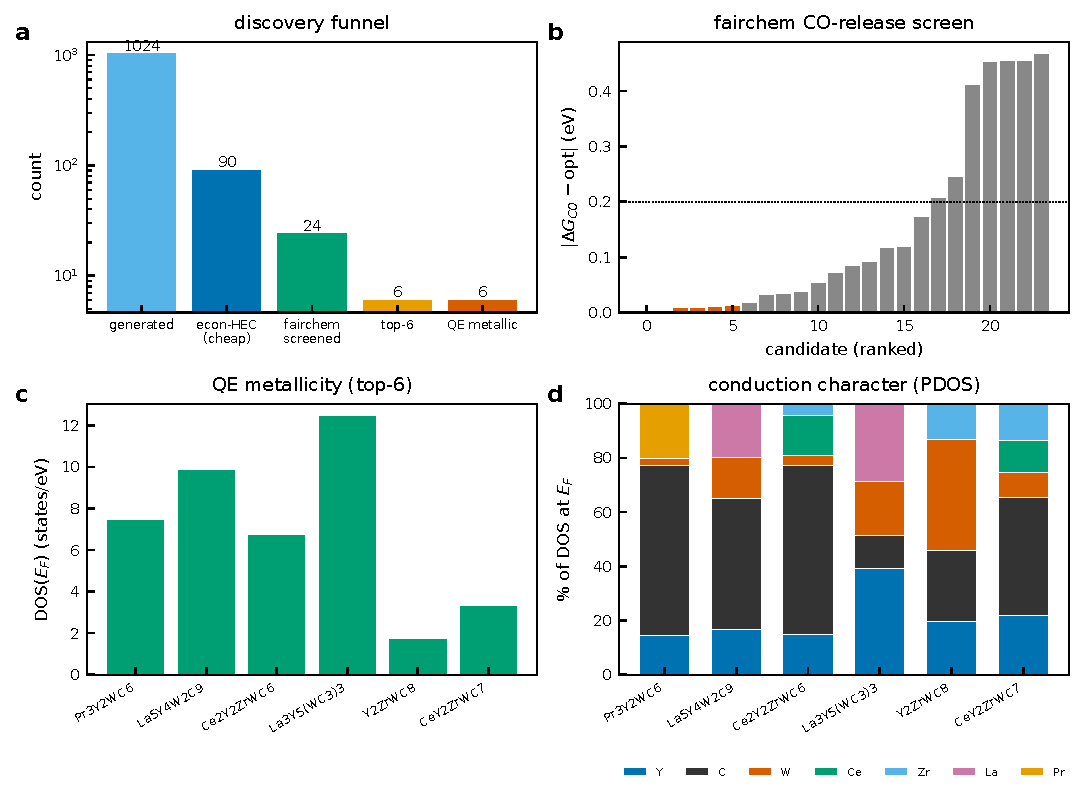
\includegraphics[width=0.92\textwidth]{fig_co2rr_pipeline_summary.pdf}
\caption{종단간 발견 종합. (a) 1024개 생성 구조에서 6개 DFT 검증 금속성 후보까지의 발견 깔때기.
(b) 스크리닝된 후보의 UMA 표면 일산화탄소 방출 디스크립터(상위 6개 강조). (c) 상위 6개의 페르미
준위 DFT 상태밀도. (d) 원소 투영 전도 특성($\Ef$에서의 원소별 DOS 비중).}
\label{fig:summary}
\end{figure}

\begin{figure}[t]
\centering
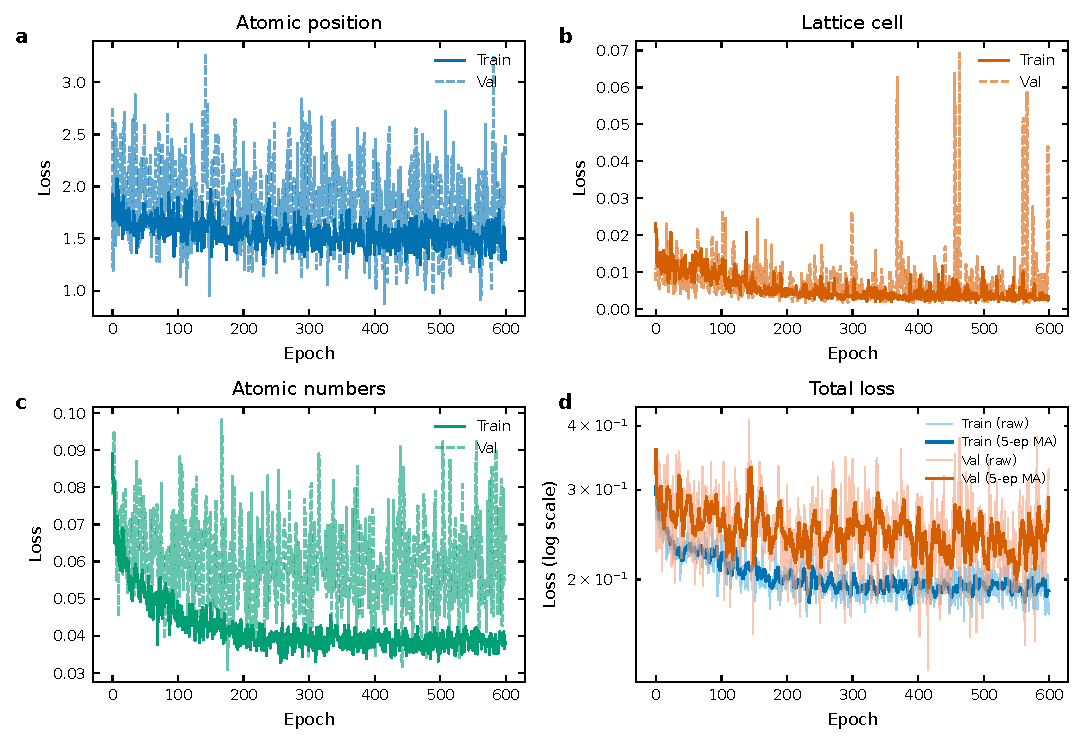
\includegraphics[width=0.78\textwidth]{fig4_composite_economic.pdf}
\caption{경제성 조건부 생성 모델의 미세조정: 600 에폭에 걸친 학습/검증 손실 및 성분별(위치, 격자,
원자종류) 손실.}
\label{fig:loss}
\end{figure}

\begin{figure}[t]
\centering
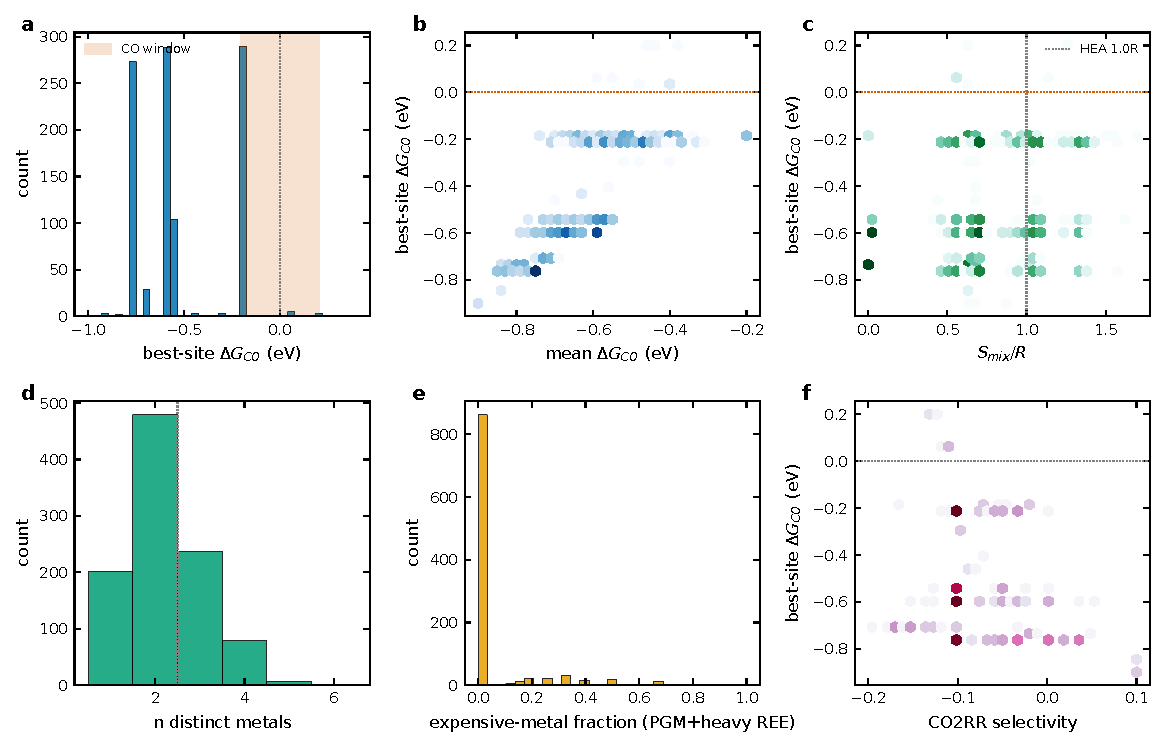
\includegraphics[width=\textwidth]{fig_co2rr_generation_stats.pdf}
\caption{생성된 카바이드 후보군의 조성 통계: (a) CO 방출 영역과 함께 본 최적 자리 CO 친화도;
(b,c) 디스크립터 상관; (d) 금속 개수 분포; (e) 고가 금속 분율(경제성 제약); (f) CO\textsubscript{2}RR
선택성.}
\label{fig:genstats}
\end{figure}

\begin{figure}[t]
\centering
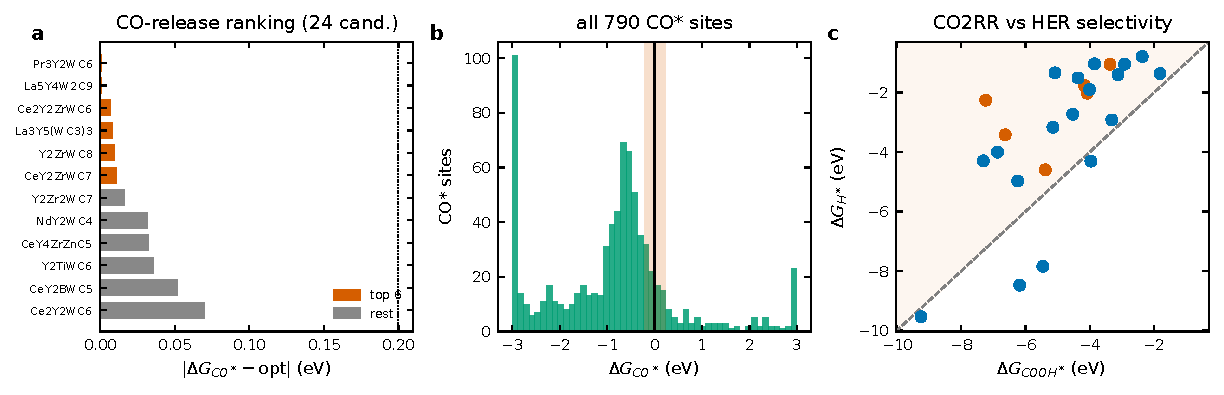
\includegraphics[width=\textwidth]{fig_co2rr_surface_screen.pdf}
\caption{UMA 표면 스크리닝: (a) 최적 자리의 CO 최적점 근접도로 순위를 매긴 후보; (b) CO 방출 영역과
함께 본 통합 $\dGCO$ 분포; (c) CO 대 H\textsubscript{2} 선택성($\dGCOOH$ 대 $\dGH$).}
\label{fig:surface}
\end{figure}

\begin{figure}[t]
\centering
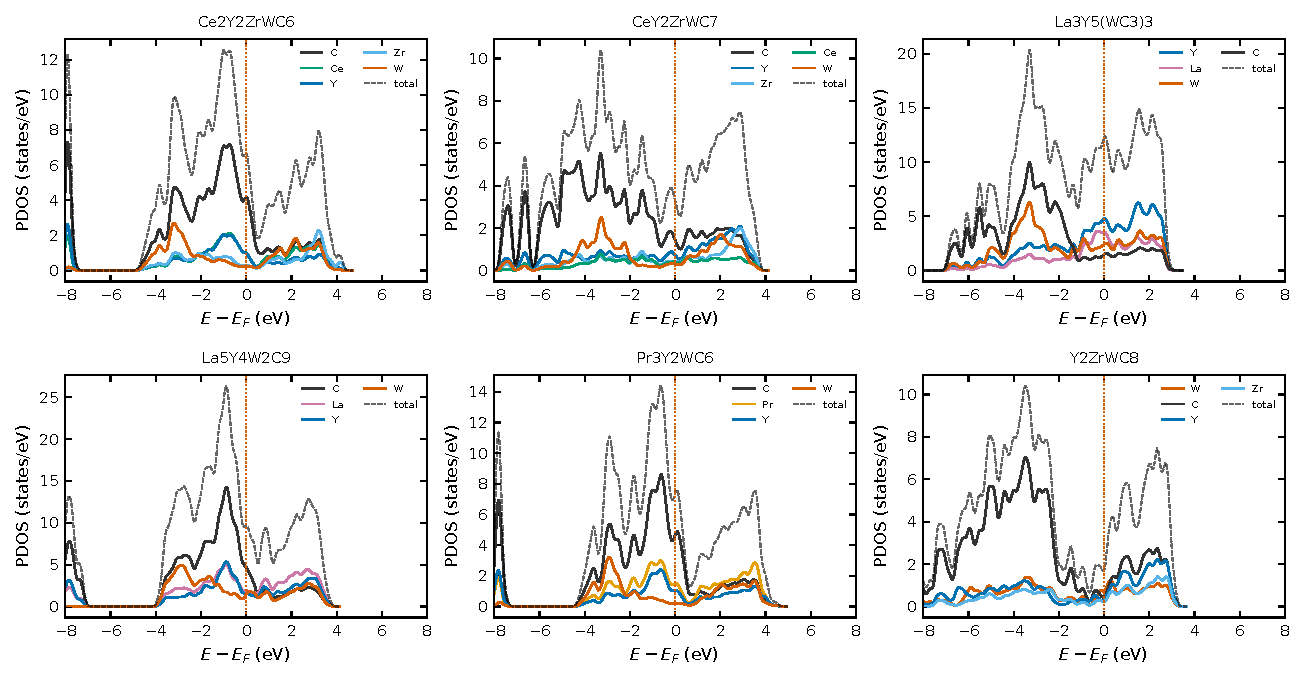
\includegraphics[width=\textwidth]{fig_co2rr_qe_pdos.pdf}
\caption{여섯 DFT 검증 후보의 원소 투영 상태밀도(PDOS), $E-\Ef$ 기준. $\Ef$(파선)에서의 유한 상태가
금속성을 확인하며, 원소별 분해가 전도 특성을 규명한다.}
\label{fig:pdos}
\end{figure}

\begin{figure}[t]
\centering
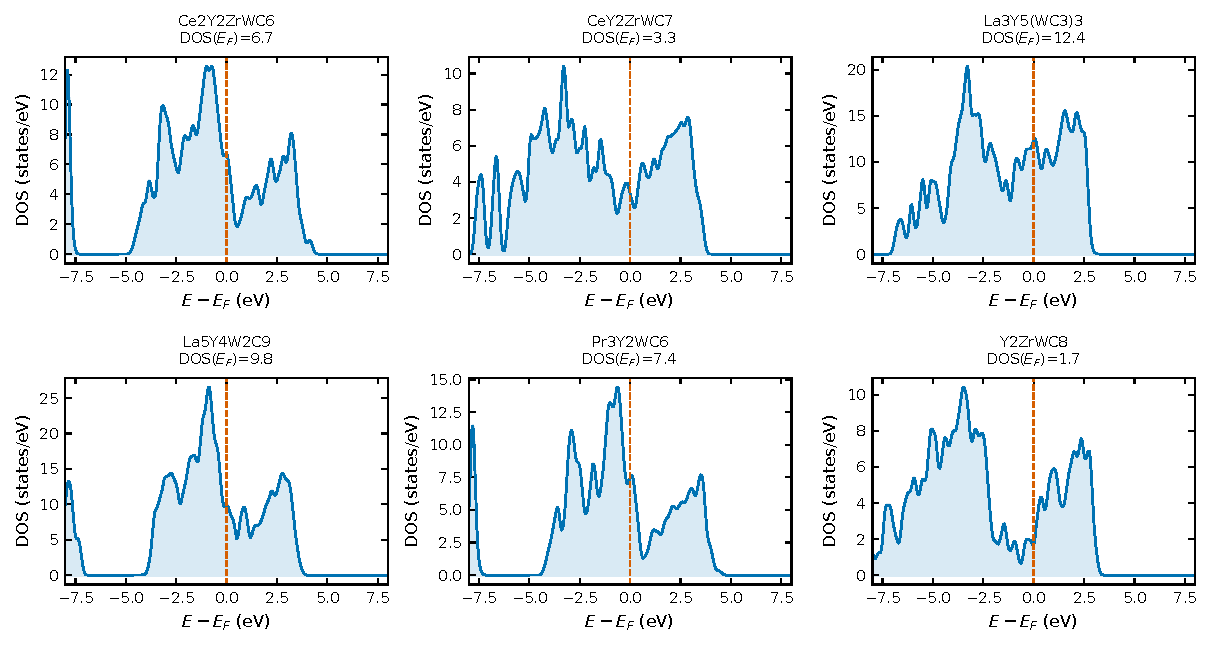
\includegraphics[width=0.9\textwidth]{fig_co2rr_qe_dos.pdf}
\caption{페르미 준위 부근 여섯 후보의 총 상태밀도(DFT, PBE).}
\label{fig:dos}
\end{figure}

% =====================================================================
\section{표면 자유에너지와 CO\texorpdfstring{$_2$}{2}RR 활성(DFT)}
\label{sec:surf-dft}
여섯 후보의 SQS 슈퍼셀에 대해, 각 결정구조에서 대칭적으로 구별되는 저지수 면을 열거하고
면마다 가장 안정한 종단을 택한 뒤, 활성이 높은 상위 세 면에 $*$CO/$*$COOH/$*$H를 전 자리에
배치하여 이완한 기하(Stage~B, UMA 스크린)를 DFT(QE) 단일점으로 재계산하였다. 총
\textbf{108개 슬랩}(6후보 $\times$ 3면 $\times$ [청정+3흡착자], 기체 기준 CO/CO$_2$/H$_2$ 포함)의
DFT 표면 자유에너지 $\dGCO$, $\dGCOOH$, $\dGH$를 완결하였다(계산 프로토콜은
\ref{ch:methods}장 참조: DFT$/\!/$UMA 단일점, $\Gamma$점, ecut 60/480~Ry, MV smearing).

\paragraph{MLIP 스크린의 DFT 검증.} DFT와 UMA(MLIP) 자유에너지는 54개 (면,흡착자) 쌍 전체에서
Pearson $r=0.973$(MAE 0.342~eV, RMSE 0.457~eV)로 강하게 상관하며, 흡착자별 MAE는 CO 0.24 /
H 0.30 / COOH 0.49~eV이다. 즉 \emph{MLIP 수준 활성 순위가 DFT에서 재현}된다. COOH의 오차가
가장 큰 것은 일부 저대칭 면에서 $*$COOH가 해리성으로 과결합($\dGCOOH \lesssim -2$~eV,
표~\ref{tab:che})하는 자리 때문이며, DFT가 이 비물리적 심우물을 부분적으로 교정한다.

\paragraph{전산 수소 전극(CHE) 자유에너지 다이어그램과 한계 전위.} 2전자 CO$_2\!\to\!$CO 경로
CO$_2+* \to *$COOH $\to *$CO $\to$ CO(g)$+*$의 두 양성자--전자 짝전달 단계
$\Delta G_1=\dGCOOH$, $\Delta G_2=\dGCO-\dGCOOH$로부터 한계 전위 $U_L=-\max(\Delta G_1,\Delta G_2)/e$를
정의한다(그림~\ref{fig:che}). \textbf{여섯 후보 모두 최적 면에서 $\dGCOOH<\dGH$}, 즉 CO$_2$
활성화가 경쟁하는 수소 발생(HER)보다 우세하여 DFT 수준에서 CO 선택성을 확인한다
(표~\ref{tab:che}). 다만 한계 전위는 두 무리로 뚜렷이 갈린다: \emph{CeY$_2$ZrWC$_7$}($U_L=-0.10$~V)와
\emph{Pr$_3$Y$_2$WC$_6$}($U_L=-0.21$~V)는 $*$COOH를 온건하게 결합하는 잘 정의된 분자 중간체를
가져 과전위가 낮은 반면, 나머지 넷은 $*$COOH를 과결합(La$_5$Y$_4$W$_2$C$_9$의 경우 $-7.8$~eV까지)하여
$*$COOH$\to*$CO 단계가 율속이 되고 겉보기 과전위가 크다. 모든 후보에서 전위 결정 단계(PDS)는
두 번째 환원 단계($*$COOH$\to*$CO)였다. 따라서 DFT는 CeY$_2$ZrWC$_7$와 Pr$_3$Y$_2$WC$_6$를
\emph{저과전위 CO$_2$RR 후보}로 특정한다.

\begin{table}[t]
\centering
\caption{후보별 최적 면의 DFT 표면 디스크립터와 CHE 한계 전위. $\Delta G$ 단위 eV, $U_L$ 단위 V vs RHE.
전 후보 $\dGCOOH<\dGH$(CO 선택적). PDS는 전위 결정 단계.}
\label{tab:che}
\small
\begin{tabular}{lcccccc}
\hline
후보 & 최적 면 & $\dGCOOH$ & $\dGCO$ & $\dGH$ & $U_L$(DFT) & $U_L$(UMA) \\
\hline
CeY$_2$ZrWC$_7$   & (011)  & $-0.47$ & $-0.37$ & $-0.42$ & $-0.10$ & $-1.80$ \\
Pr$_3$Y$_2$WC$_6$ & (010)  & $-0.63$ & $-0.42$ & $-0.23$ & $-0.21$ & $-0.66$ \\
La$_3$Y$_5$(WC$_3$)$_3$ & (101) & $-1.28$ & $+0.13$ & $-0.34$ & $-1.40$ & $-2.19$ \\
Ce$_2$Y$_2$ZrWC$_6$ & (101) & $-3.12$ & $-0.81$ & $-1.38$ & $-2.31$ & $-2.99$ \\
La$_5$Y$_4$W$_2$C$_9$ & (111) & $-2.40$ & $-0.03$ & $-0.04$ & $-2.37$ & $-2.95$ \\
Y$_2$ZrWC$_8$     & (100)  & $-2.19$ & $+0.22$ & $-0.30$ & $-2.41$ & $-2.50$ \\
\hline
\end{tabular}
\end{table}

\begin{figure}[t]
\centering
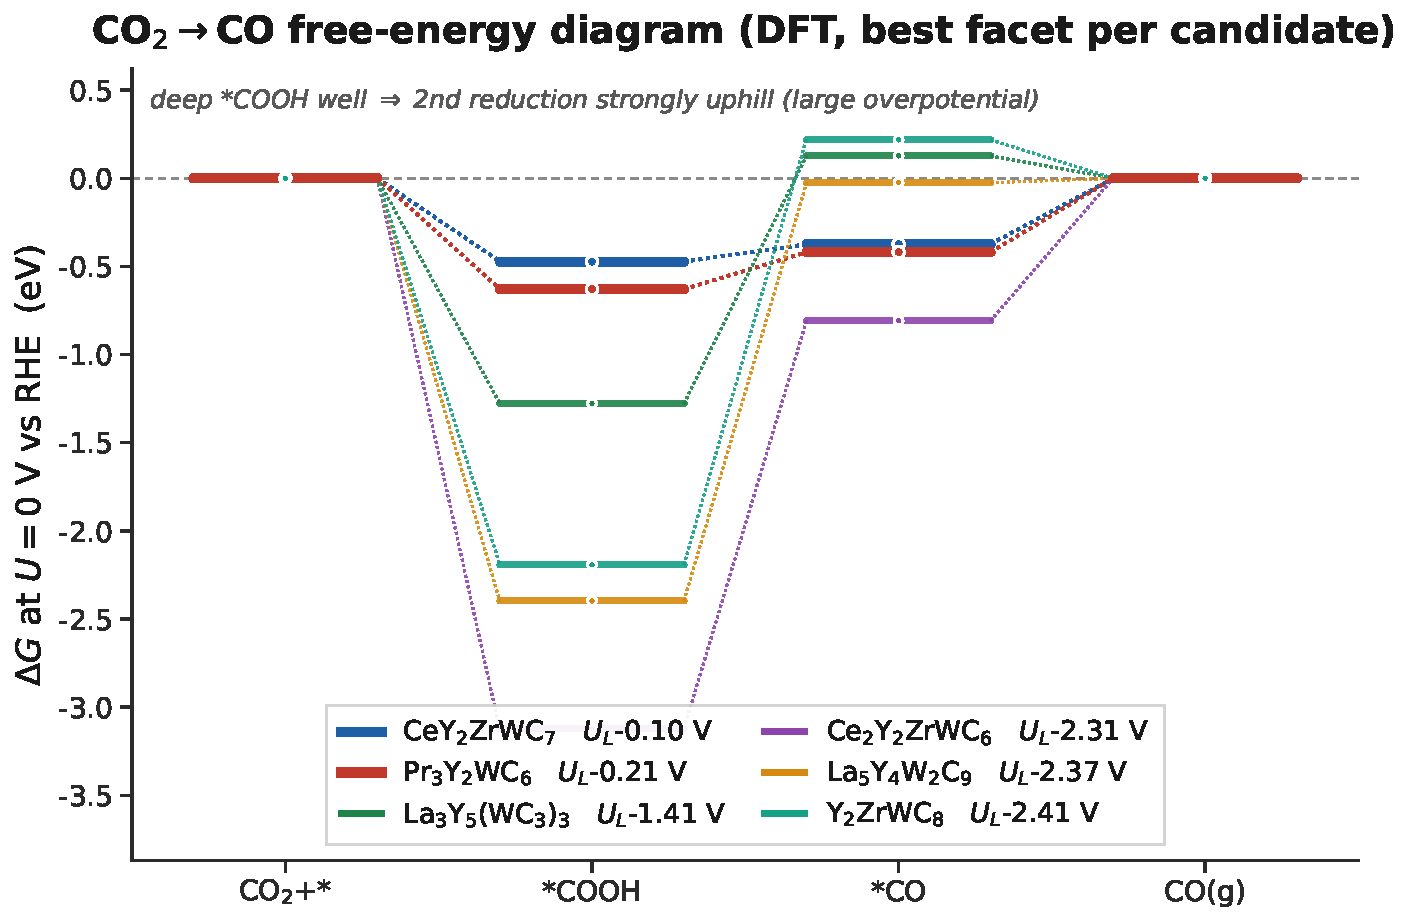
\includegraphics[width=0.92\textwidth]{fig_co2rr_che_diagram.pdf}
\caption{여섯 후보의 CO$_2\!\to\!$CO 전산 수소 전극(CHE) 자유에너지 다이어그램($U=0$ vs RHE,
후보별 최적 면). 낮은 과전위 후보(CeY$_2$ZrWC$_7$, Pr$_3$Y$_2$WC$_6$)는 $*$COOH가 온건한 중간
상태인 반면, 나머지는 $*$COOH 심우물로 두 번째 환원이 강하게 흡열이다.}
\label{fig:che}
\end{figure}

\paragraph{$d$-밴드 중심과 흡착 디스크립터.} 각 후보의 저장된 Kohn--Sham 파동함수를 원자 궤도로
투영(projwfc)해 전이금속 $d$-투영 상태밀도로부터 $d$-밴드 중심 $\varepsilon_d$($\Ef$ 기준)를
산출하였다(그림~\ref{fig:dband}). 금속 평균 $\varepsilon_d$는 Pr$_3$Y$_2$WC$_6$($-0.48$~eV)에서
Y$_2$ZrWC$_8$($-1.46$~eV)에 걸치며, 원소별로는 W의 중심이 가장 깊고($-1$$\sim$$-2.3$~eV) 희토류
5$d$와 Zr가 $\Ef$에 더 가깝다. $d$-밴드 모형과 일관되게, 중심이 $\Ef$에 가까운($\varepsilon_d$ 높은)
후보일수록 CO를 더 강하게 결합하는 경향을 보여, 전도 특성과 흡착 디스크립터를 연결한다.

\begin{figure}[t]
\centering
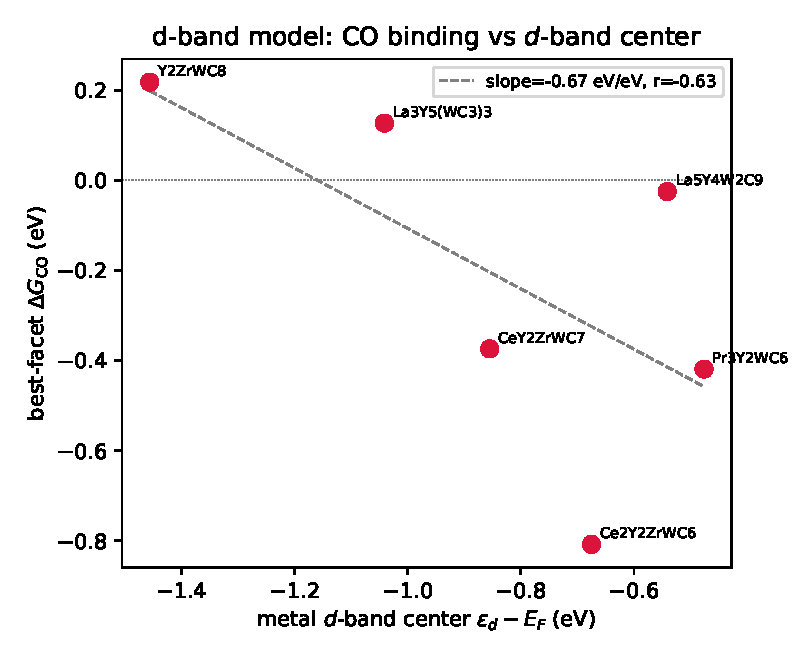
\includegraphics[width=0.62\textwidth]{fig_co2rr_dband_vs_dGCO.pdf}
\caption{금속 $d$-밴드 중심 $\varepsilon_d-\Ef$ 대 최적 면 $\dGCO$. $d$-밴드가 높을수록 CO 결합이
강해지는 경향(추세선)으로 전도 특성과 흡착을 연결한다.}
\label{fig:dband}
\end{figure}

% =====================================================================
\section{생성에너지와 볼록 껍질 안정성(DFT + Materials Project)}
\label{sec:hull}
여섯 후보의 벌크 생성에너지를 동일 QE-PBE 수준의 원소 참조(W bcc, Zr/Y hcp, La/Ce/Pr fcc,
C 다이아몬드; vc-relax)로부터 산출하고, 같은 화학공간의 경쟁상(Materials Project GGA 엔트리,
모든 하위계 포함)으로 볼록 껍질을 구성하여 껍질 위 에너지 $E_{\mathrm{hull}}$를 평가하였다
(표~\ref{tab:hull}). 원소 기준 상쇄로 QE와 MP(VASP) 생성에너지 차이는 대부분 소거되며, 잔차는
$\sim$0.1~eV/atom 수준으로 추정한다. 여섯 후보의 $E_{\mathrm{hull}}$는 $+0.15\!\sim\!+0.36$~eV/atom로,
0~K 엔탈피 기준 \emph{준안정}이다 --- 이는 고엔트로피 카바이드에서 전형적이다(엔트로피 안정화
물질이지 엔탈피 바닥상이 아님). 이상 배열 엔트로피에 의한 안정화 $-T\Delta S_{\mathrm{mix}}$는
1800~K에서 $-0.05\!\sim\!-0.10$~eV/atom로 껍질 거리를 줄이지만 단독으로 완전히 상쇄하지는 못하며
(교차 온도 $T^\ast\approx 3000\!\sim\!12000$~K), 따라서 실제 합성 가능성은 진동 엔트로피, 비이상
혼합 엔탈피, 고온 급랭에 의한 \emph{동역학적 포획}, 그리고 위 방법론적 불확실성에 함께 의존한다.
요컨대 이 ML-생성 후보들은 합성 가능성이 자명하지 않은 준안정 상이며, 이는 \ref{ch:experiment}장의
합성·상순도 시험(XRD/XPS)을 직접 동기화한다.

\begin{table}[t]
\centering
\caption{DFT 생성에너지(QE 원소 참조)와 MP 볼록 껍질 대비 껍질 위 에너지, 이상 배열 엔트로피
안정화. $E_f, E_{\mathrm{hull}}$ 단위 eV/atom. $T^\ast$는 이상 엔트로피가 껍질 거리를 상쇄하는 온도.}
\label{tab:hull}
\small
\begin{tabular}{lcccc}
\hline
후보 & $E_f$(QE) & $E_{\mathrm{hull}}$ & $-T\Delta S_{\mathrm{mix}}$(1800\,K) & $T^\ast$(K) \\
\hline
La$_3$Y$_5$(WC$_3$)$_3$ & $-0.087$ & $+0.154$ & $-0.091$ & 3050 \\
La$_5$Y$_4$W$_2$C$_9$   & $-0.024$ & $+0.191$ & $-0.088$ & 3890 \\
CeY$_2$ZrWC$_7$         & $-0.118$ & $+0.223$ & $-0.086$ & 4660 \\
Pr$_3$Y$_2$WC$_6$       & $+0.046$ & $+0.265$ & $-0.078$ & 6080 \\
Ce$_2$Y$_2$ZrWC$_6$     & $-0.067$ & $+0.309$ & $-0.103$ & 5390 \\
Y$_2$ZrWC$_8$           & $+0.072$ & $+0.360$ & $-0.054$ & 12040 \\
\hline
\end{tabular}
\end{table}

% =====================================================================
\section{정밀 검증(Stage C): 상위 후보의 DFT 이완과 $k$-수렴}
\label{sec:stagec}
지금까지의 표면 자유에너지는 UMA로 이완한 기하에 대한 DFT 단일점(DFT$/\!/$UMA, $\Gamma$)이다. 활성
상위 두 후보(CeY$_2$ZrWC$_7$, Pr$_3$Y$_2$WC$_6$)에 대해 그 활성 면에서 청정슬랩·$*$CO·$*$COOH·$*$H를
\emph{완전 이온 이완}(GPU QE, 하부 절반 고정, $\Gamma$)하여 헤드라인 결과를 정밀화하였다.

\paragraph{$k$-점 수렴.} 대칭이 없는 50원자급 슬랩은 16~GB VRAM에서 $k>\Gamma$가 실행 불가하나,
$\Delta G$는 동일 셀·동일 $k$의 차분이라 유한-$k$ 오차가 상쇄된다. 36원자 슬랩에서 $\Gamma$ 대
$2{\times}1{\times}1$ 흡착 자유에너지 차는 $\Delta G_{\rm CO}$ 0.01~eV, $\Delta G_{\rm COOH}$ 0.11~eV로,
슬랩 절대 에너지가 $\sim$0.7~eV 이동함에도 차분은 안정하여 $\Gamma$ 수준 $\Delta G$를 정당화한다.

\paragraph{이완이 상위 순위를 정제한다.} 완전 이완 결과, \textbf{CeY$_2$ZrWC$_7$의 저과전위가 견고}하게
확인되었다: $\Delta G_{\rm CO}=-0.09$~eV(거의 완벽한 열중성; 단일점 $-0.37$에서 이완으로 개선),
$U_L=-0.15$~V(단일점 $-0.10$과 0.05~V 차). 반면 \textbf{Pr$_3$Y$_2$WC$_6$의 단일점 활성은 견고하지
않았다}: 이완 시 활성 면의 $*$COOH가 \emph{해리}되어(이완 기하에서 C--O 결합 하나가 3.3~\AA로 끊김,
$*$CO$+*$O로 분해) $\Delta G_{\rm COOH}=-3.66$~eV의 심우물로 떨어지며 $U_L$이 $-3.1$~V로 악화된다. 즉
Pr$_3$Y$_2$WC$_6$의 낮은 단일점 $U_L$은 UMA 기하의 인공산물이었다. 양 후보 모두 $*$COOH의 해리 경향을
보이나, CeY$_2$ZrWC$_7$에서는 분해 산물의 결합이 온건하여 활성이 유지된다. 따라서 \emph{이완에 무관하게
견고한 $\Delta G_{\rm CO}$가 신뢰할 활성 디스크립터}이며, 이 기준에서 \textbf{CeY$_2$ZrWC$_7$($\Delta
G_{\rm CO}\!=\!-0.09$~eV)가 유일하게 이상적인 CO 발생 후보}로 부각된다. $*$COOH 해리의 미시적 경로와
미소동역학은 후속 과제다.

% =====================================================================
\section{최종 탄화물의 전산 검증 현황과 남은 과제}
\label{sec:outstanding}
Stage A$'$(\ref{ch:methods}장)에서 고엔트로피 숏리스트의 특수 준무작위 구조들을 암염형·육방정 골격 위
명시적 무질서 슈퍼셀로 구성(금속 부격자 쌍상관 오차 최소화)하였고, 이들은 위 표면 연구
(\ref{sec:surf-dft}절)의 기질이다. 본 연구의 \emph{최종 산물은 설계 관문 A1--A4를 모두 통과한 3종의
Ti계 암염형 카바이드}(hec3-MoTiZr/CrTiV/CrTiZr)이므로, 여기서는 \textbf{이 3종에 대한 제일원리 검증
현황}을 정리한다.

\paragraph{완료된 검증(3 최종 탄화물).}
\begin{itemize}[nosep]
\item \textbf{이중목표 표면 자유에너지·한계 전위}: 면별 DFT$/\!/$UMA로 CO 발생($|\dGCO|<0.3$)과
H 반발($\dGH>0$)을 동시 확인하고 $U_L$을 산출(표~\ref{tab:dual}, 그림~\ref{fig:summaryB}b).
\item \textbf{대표 후보 완전 이완}: hec3-MoTiZr (100)을 GPU DFT로 완전 이완하여 선택성을 재확인
($\dGH\!=\!+0.57$; CO는 Mo ontop 약결합이라 방출)하고 $U_L$을 $-0.40$~V로 정정(\ref{sec:stagec}절,
그림~\ref{fig:moTiZr}).
\item \textbf{볼록 껍질 안정성}: QE-PBE 생성에너지 + Materials Project 껍질로 3종 모두 캠페인 A보다
안정하며 MoTiZr는 사실상 껍질 위($E_{\mathrm{hull}}\!\approx\!-0.02$)임을 확인(표~\ref{tab:comp},
\ref{sec:hull}절).
\item \textbf{벌크 금속성·전도 특성}: QE 벌크 DOS/PDOS로 3종 모두 금속성(DOS($\Ef$)
$21$--$35$~states/eV)이며 CO를 결합하는 6족 금속(Mo/Cr)이 $\Ef$ 상태를 지배함을 확인
(그림~\ref{fig:summaryB}c,d).
\item \textbf{다중탄소 분기}: (100) 표면에서 $*$CO의 세 운명(CO 방출 / C1 $*$CHO / C2 $*$OCCO)을
계산, C2 짝지음이 안정화되어 실험 에탄올과 정합함을 보임(그림~\ref{fig:cheher}, \ref{sec:tandem}절).
\end{itemize}

\paragraph{남은 제일원리 과제(3 최종 탄화물).}
\begin{itemize}[nosep]
\item \tbc{hec3-CrTiV·CrTiZr의 완전 이완(현재 단일점)으로 $U_L$ 확정}
\item \tbc{측면 상호작용을 포함한 \emph{피복 의존} 미시동역학과 반응-확산 국소 pH 모형}
\item \tbc{투영 결정-궤도(COHP/COOP, LOBSTER) 결합 세기 분석으로 6족--CO 결합의 정량화}
\item \tbc{작동 전위에서 \emph{카바이드} 표면 Pourbaix(격자 안정화 포함)로 산화막·OH 피독 여유 정량}
\item \tbc{명시적 C--C 짝지음/에탄올 경로(전이상태·장벽)의 제일원리 계산}
\end{itemize}

\paragraph{캠페인 A(희토류) 진단의 역할.} 위와 별개로, 캠페인 A의 6개 희토류 후보에 대해서도 활성 면
$*$COOH \emph{해리성 과결합}(Pr$_3$Y$_2$WC$_6$에서 C--O가 3.3~\AA로 끊겨 $*$CO$+*$O로 분해,
\ref{sec:stagec}절)과 작동 전위 \emph{평균장 피복률} 포화($\theta_{*\mathrm{COOH}}\!\approx\!0.87$--$1.0$)를
계산하였다. 이는 최종 후보의 검증이 아니라, \emph{활성-우선(제약 없는) 탐색이 기계적으로도 무리}임을
드러내는 \textbf{반례 증거}다 --- 이 후보군은 다음 절의 제조 가능성 관문(\ref{sec:ree-stability}절)에서
탈락하며, 그 결과가 캠페인 B의 제조 가능성 제약(A3)을 정당화한다. 따라서 희토류 후보에 대한 추가
전산(예: COHP, 피복 의존 DFT)은 \emph{불필요}하며, 남은 과제는 위 3종의 최종 탄화물에 집중한다.

% =====================================================================
\section{제조 가능성 관문: 희토류의 수용액 산화·용출과 활성점 피독}
\label{sec:ree-stability}
캠페인 A의 숏리스트는 활성·안정성·경제성으로 선별되었을 뿐, 설계 공리 \textbf{A3(제조 가능성)}에
대해서는 검증되지 않았다. 본 절은 이 관문을 제일원리 표면 열역학과 실험열역학 Pourbaix로 반증
가능하게 시험한다. \emph{결론부터, 캠페인 A 후보군은 이 관문을 통과하지 못한다} --- 그리고 이 사실이
캠페인 B에서 제조 가능성을 생성 제약으로 승격시키는 근거가 된다. 숏리스트는 La, Ce, Pr 등 경희토류를
금속 부격자에 포함한다. 이들은 산소친화도가 매우 커,
표준 환원 전위가 $M^{3+}\!+\!3e^-\!\to\!M$에 대해 La $-2.38$, Ce $-2.34$, Pr $-2.35$, Y $-2.37$~V(SHE)로
CO$_2$RR 작동창($\approx -0.5\!\sim\!-1.1$~V vs RHE)보다 훨씬 음(陰)이다. 즉 \emph{금속 상태}의
희토류는 열역학적으로 산화·용해(예: $M^{3+}_{(aq)}$ 또는 $M(OH)_3$/$M_2O_3$)로 강하게 기운다.
따라서 핵심 물음은 ``카바이드 격자의 안정화가 이 구동력을 상쇄해 활성점을 보존하는가''이며,
이는 세 층위의 제일원리 계산으로 반증 가능하게 시험할 수 있다.

\paragraph{(1) 표면 Pourbaix / $*$O,$*$OH 피복(활성점 피독의 직접 시험).} $*$CO/$*$COOH/$*$H와
동일한 슬랩·CHE 틀에서 $*$O, $*$OH의 흡착 자유에너지를 계산한다:
$\Delta G_{*\mathrm{OH}}=G_{*\mathrm{OH}}-G_*-(G_{\mathrm{H_2O}}-\tfrac12 G_{\mathrm{H_2}})+eU$,
$\Delta G_{*\mathrm{O}}=G_{*\mathrm{O}}-G_*-(G_{\mathrm{H_2O}}-G_{\mathrm{H_2}})+2eU$.
주어진 $(U,\mathrm{pH})$에서 자유에너지를 최소화하는 표면 종을 취해 \emph{표면 Pourbaix 도표}를
작성하면, 작동 전위에서 표면이 청정/$*$H 피복인지 $*$OH/$*$O로 피독되는지 판정된다. 특히 희토류
자리에서 $*$OH가 $*$CO/$*$COOH보다 강하게 결합하면 활성점 피독을 예측한다. \emph{완화 요인}:
CO$_2$RR은 음극(환원) 전위에서 작동하므로 열역학적으로 산화가 억제되어(음극 방어) 정상 작동 중
피독 위험은 낮고, 위험은 개회로/기동 및 국소 알칼리화 시 최대가 된다 --- Pourbaix 도표가 이
전위·pH 의존성을 정량화한다.

\emph{$*$O/$*$OH 스크린(UMA).} Stage~B 파이프라인에 $*$O, $*$OH를 흡착자로 추가해 여섯 후보의
전 면·전 자리(후보당 120$\sim$306 자리)를 스크린하였다. 최강 결합 자리의 자유에너지는
$\Delta G_{*\mathrm{OH}}(0)=-2.4\!\sim\!-7.0$~eV, $\Delta G_{*\mathrm{O}}(0)=-1.2\!\sim\!-8.8$~eV로
$*$CO($\Delta G_{\rm CO}\!\approx\!0$)보다 훨씬 강하여, 이 희토류-카바이드 표면의 큰 산소친화도를
보인다. 이는 산화 피복의 열역학적 \emph{경향}을 시사하나, 실제 작동 중 정지상태는 반응 중간체
$*$COOH를 포함한 같은-면 비교로 판정해야 하며(아래 DFT 정정 참조), 이때 산화가 아니라 $*$COOH가
우세함이 드러난다.

\emph{활성 면 같은-면 완전 Pourbaix(DFT, 여섯 후보 완결).} 정지상태를 엄밀히 판정하려면 경쟁
흡착종을 \emph{같은 면}에서, 특히 CO$_2$RR 반응 중간체 $*$COOH를 포함해
($\Delta G_{*\mathrm{COOH}}(U)=\Delta G_{*\mathrm{COOH}}(0)+eU$) 비교해야 한다. 이를 위해 각 후보의
\emph{활성 면}(최소 $U_L$ 면, 표~\ref{tab:che})에서 $*$O/$*$OH를 QE로 재계산해(24 슬랩, GPU;
La-rich·대형 슬랩은 CPU 폴백) $*$CO/$*$COOH/$*$H와 동일 면에서 결합하였다. \textbf{활성 면의
$*$OH/$*$O 결합은 최악 면보다 훨씬 약하다}($\Delta G_{*\mathrm{OH}}=-0.8\!\sim\!-1.6$~eV, 일부
$\Delta G_{*\mathrm{O}}\!\gtrsim\!0$) --- 즉 실제 반응 면은 산소친화도가 낮다. 여섯 후보 같은-면
Pourbaix(그림~\ref{fig:pourbaix})의 결론: \textbf{작동 전위($-0.3\!\sim\!-1.0$~V vs RHE)에서 여섯
후보 모두 반응 중간체 $*$COOH가 정지상태}이며(-0.6~V 이하는 6/6, $-0.3$~V는 5/6; La$_3$Y$_5$만
$-0.6$~V에서 전환), $*$O/$*$OH 산화 피복은 \emph{개회로 부근($\sim\!0$~V)의 과도적 상태}에 국한된다.
따라서 \emph{음극 작동 조건에서는 산화 피독이 아니라 $*$COOH(작동 상태)가 지배}하며, 앞선
``전면 피독'' 판정은 (i) $*$COOH 누락과 (ii) 면 혼합에 기인한 인공산물이었다. 산화 위험은 실재하나
그 무대는 \emph{기동/개회로}이고, 후보 차별화의 실질 축은 산화가 아니라 $*$COOH 결합 세기(활성,
표~\ref{tab:che})다. UMA와의 일치는 활성 면(약결합)에서 $r=0.74$(MAE 0.60~eV)로 최악 면($r=0.99$)보다
낮은데, 이는 약하게 결합하는 자리에서 MLIP 신뢰도가 떨어짐을 뜻하며 DFT(기준)는 오히려 \emph{더 약한}
결합(더 낮은 산소친화도)을 준다. 교차 검증은 \ref{ch:experiment}장의 XPS 산화 상태·용출 후분석과
in-situ FT-IR($*$COOH/$*$CO 밴드)로 수행한다.

\begin{figure}[t]
\centering
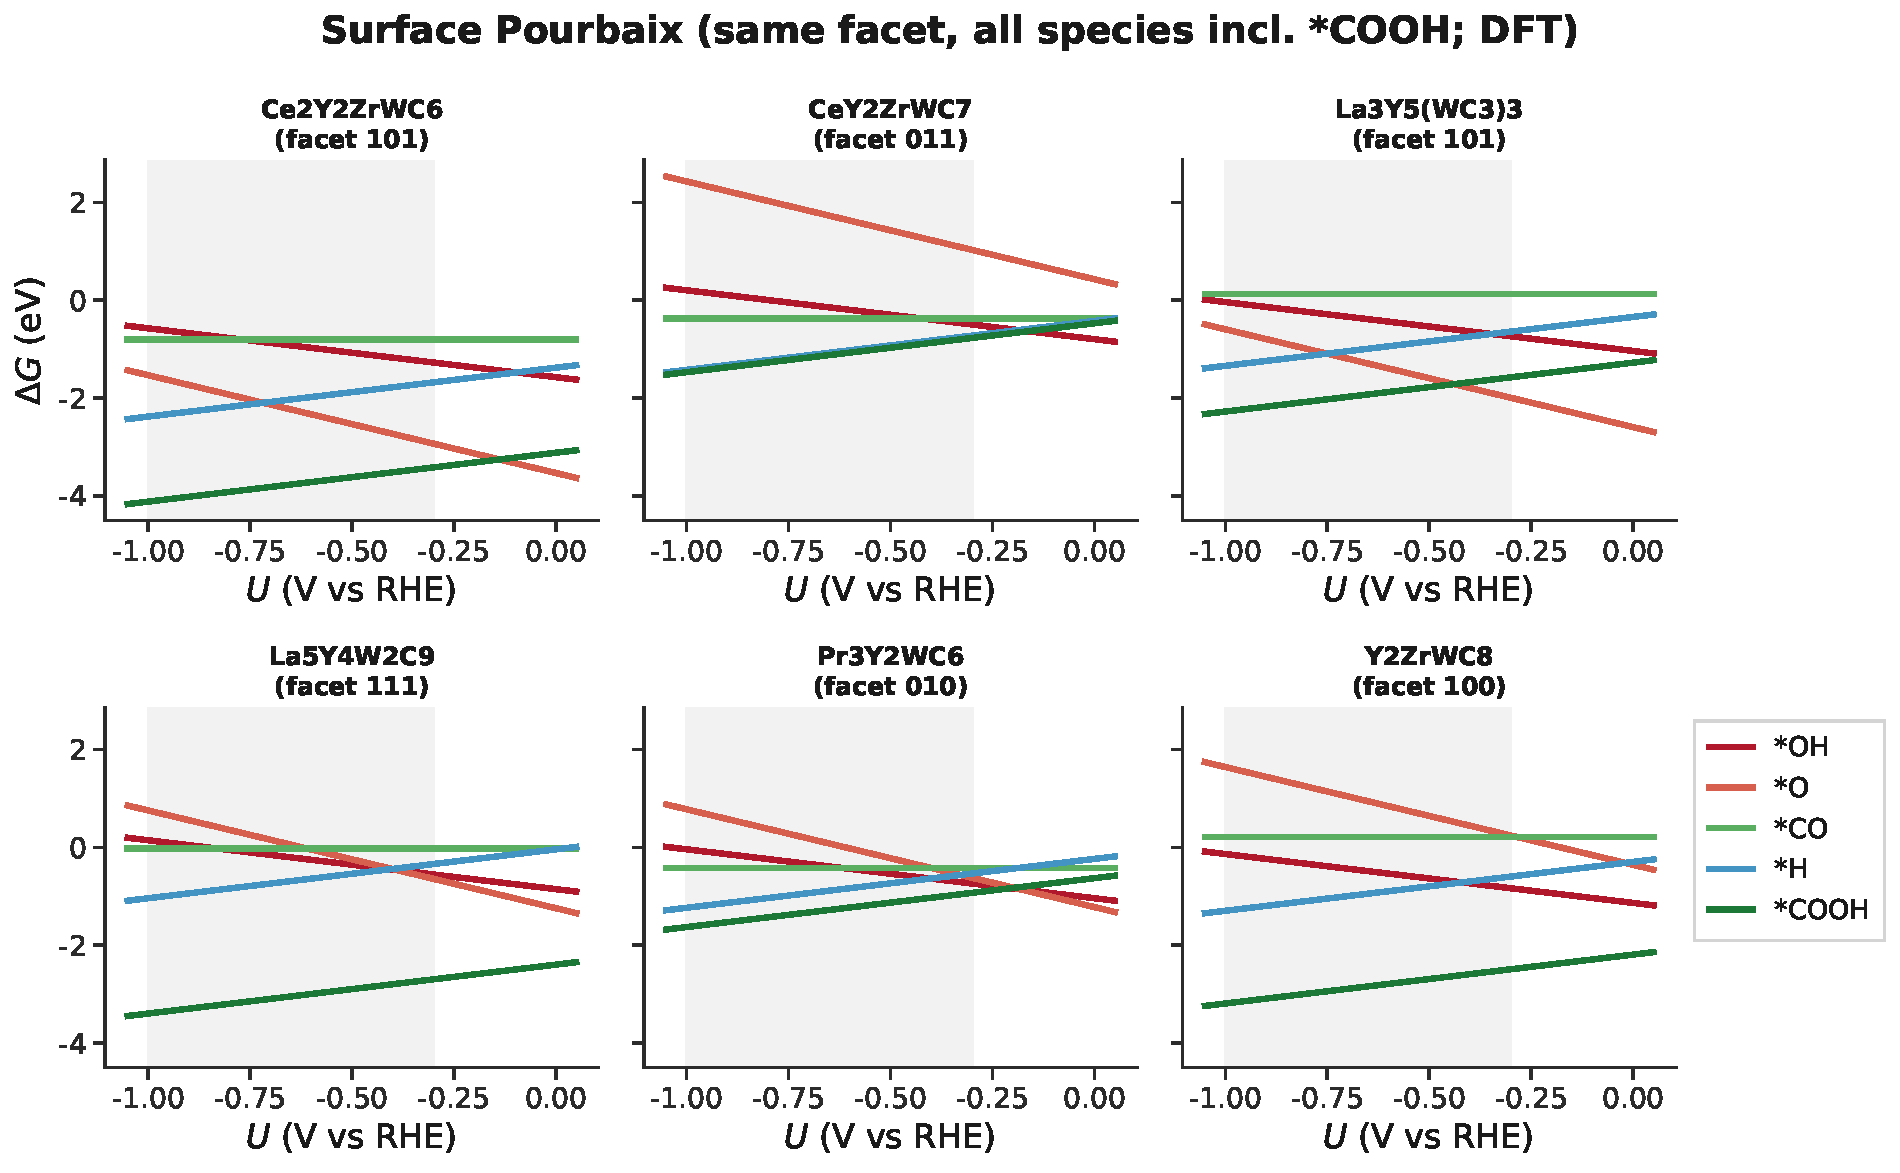
\includegraphics[width=\textwidth]{fig_co2rr_surface_pourbaix_dft.pdf}
\caption{여섯 후보의 활성 면 같은-면 완전 표면 Pourbaix(DFT, $*$COOH 포함). 각 흡착종 $\Delta G$의
전위 의존성; 작동창(음영)에서 최저 $\Delta G$ 종이 정지상태다. 작동 전위 전역에서 반응 중간체
$*$COOH(녹색)가 우세하고 산화 종($*$OH/$*$O, 적색)은 개회로 부근에만 나타나, 작동 중 산화 피독이
아님을 보인다.}
\label{fig:pourbaix}
\end{figure}

본 계산은 Stage~B/Phase~A 파이프라인($*$O,$*$OH를 흡착자로 추가; 스크립트
\texttt{co\_surface\_screen}의 \texttt{-{}-adsorbates OH,O} 및 \texttt{61\_surface\_pourbaix.py})을
재사용한다.

\paragraph{(2) 벌크 Pourbaix / 용출 열역학(수행 완료).} 구성 금속이 작동 조건에서 금속(면역)으로
남는지, 고체 산화물/수산화물로 부동태화되는지, 아니면 용존 이온으로 용출되는지를 \emph{실험 열역학}
Pourbaix로 판정하였다(수용액 이온·기준 산화물 $\Delta G_f$는 Materials Project 이온 참조(Wagman/NBS),
수산화물은 CRC/Wagman 표; pymatgen \texttt{PourbaixDiagram}으로 Nernst 전위·pH 의존성 계산). CO$_2$RR
조건(pH~7, 국소 음극 알칼리화 pH~10 포함; $U=0\!\sim\!-1.1$~V vs RHE)에서 결과는(표~\ref{tab:pourbaix}):
\textbf{어느 금속도 작동 전위에서 면역(금속 안정)이 아니다}(음극 바이어스 하의 W 제외). La·Ce·Zr은
수산화물막으로 \emph{부동태화}되고, Pr·Y는 이온으로 \emph{용출}되며(단 Y는 국소 알칼리 pH에서 부동태화),
W는 개회로에서 텅스텐산염(WO$_4^{2-}$)으로 용해되나 음극 바이어스에서 면역이다. 즉 벌크 열역학은
\emph{개회로/기동 시 산화(부동태화 또는 용출)}를 예측하여 표면 결과(작동 전위=$*$COOH 정지상태)와
정합한다. \emph{유의}: 이는 \emph{순금속} 기준이라 카바이드 격자 안정화(\ref{sec:hull}절의 생성에너지)를
포함하지 않은 \emph{용출 상한}이며, 실제 카바이드는 더 안정하다. 수산화물 $\Delta G_f$의 표값 불확실성
($\sim$수십 kJ/mol)도 정성 판정에는 영향이 작다.

\begin{table}[t]
\centering
\caption{구성 금속의 벌크 수용액 Pourbaix(실험 열역학) 판정. CO$_2$RR 작동창(pH~7) 및 국소 알칼리
(pH~10)에서 안정상. 면역=금속, 부동태=고체 산/수산화물, 용출=용존 이온. \emph{순금속 기준(용출 상한)}.}
\label{tab:pourbaix}
\small
\begin{tabular}{lcc}
\hline
금속 & pH~7 ($0\!\sim\!-1.1$~V RHE) & 국소 pH~10 \\
\hline
La & 부동태 (La(OH)$_3$) & 부동태 \\
Ce & 부동태 (Ce(OH)$_3$) & 부동태 \\
Pr & \textbf{용출 (이온)} & 용출 \\
Y  & \textbf{용출 (Y$^{3+}$)} & 부동태 \\
Zr & 부동태 (Zr(OH)$_4$) & 부동태 \\
W  & 개회로 용출 / 바이어스 하 면역 & 면역 \\
\hline
\end{tabular}
\end{table}

\paragraph{(3) 명시적 표면 산화·탄소 공공 형성 에너지(선택).} 표면 C를 O로 치환하거나 산소
과층(overlayer)을 형성하는 에너지, 표면 탄소 공공 형성 에너지를 DFT로 계산해, 격자가 초기 산화에
대해 갖는 국소 장벽을 (1)의 열역학에 보강한다.

이 세 시험은 함께 ``희토류가 격자에 묶여 있어도 전해질 노출 시 산화·용출로 활성점을 덮을 위험''을
정량적·반증 가능하게 규명한다. 위 (1) 표면 $*$O/$*$OH Pourbaix와 (2) 벌크 용출 Pourbaix는 \emph{수행
완료}되어 일관된 그림을 준다: \textbf{작동 음극 전위에서는 표면이 $*$COOH 정지상태이나, 개회로/기동
조건에서는 벌크 금속이 부동태화(La·Ce·Zr)되거나 용출(Pr·Y)}된다. 실험적으로는 시험 전후 XPS(표면
산화 상태)와 용출액 ICP-MS, in-situ 라만/SEIRAS의 $M$--O 밴드로 교차 검증한다(\ref{ch:experiment}장).

% =====================================================================
\section{캠페인 B --- 이중 활성점 기반 산-안정 카바이드 설계}
\label{sec:campaignB}\label{sec:ree-free}
캠페인 B는 네 설계 공리(A1--A4)를 모두 부과한다. 캠페인 A와의 결정적 차이는 두 가지 --- 제조
가능성(A3)을 탐색 공간에 내재화하고, 선택성(A2)을 명시적 CO/H \emph{이중 활성점} 기준으로 강화한
것이다. 희토류를 배제하는 근거는 \emph{서로 독립된 두 명제}이며, 이를 분리해 두는 것이 중요하다.

\emph{(근거 1 --- 제조 가능성.)} 본 카바이드의 합성 경로는 산화물 전구체를 Mg/Ca로 금속열환원한 뒤
부산물 산화물(MgO/CaO)을 \emph{산-침출}로 제거한다. 이 필수 침출 단계에서 희토류는 전량 용해되어
(La/Ce/Pr/Y의 표준 환원 전위가 매우 음, $M^{3+}$ 수화가 강함; \ref{sec:ree-stability}절), 캠페인 A의
후보군은 \emph{작동 이전 합성 단계에서 이미 제조 불가}가 된다. 이는 활성점 물리와 무관한 \emph{합성}
제약이다. \emph{(근거 2 --- 불필요성.)} 뒤에서 보이듯 CO 방출·H 반발이라는 이중 활성점 거동은
전이금속의 \emph{원자가전자농도(VEC)} 효과로 설명되며(저 VEC = 4족-rich = H 반발), 희토류를 전혀
요구하지 않는다 --- 오히려 희토류(3족·$f$-전자)는 이 VEC-제어 영역 밖에 놓인다. 즉 희토류는 제조상
배제되어야 하고, \emph{동시에} 활성점 설계상 불필요하다. 두 근거는 독립적으로 성립하므로, 어느 하나가
약화되어도 배제 결론은 유지된다.

\paragraph{탐색 공간과 조건화 라벨.} 따라서 캠페인 B는 금속 부격자를 \emph{산-침출을 견디는} 4/5/6족
전이금속 \{Ti, Zr, Hf, V, Nb, Ta, Cr, Mo, W\}과 비금속 \{C, B, N\}으로 한정하고(경질 화이트리스트,
\texttt{carbidemattergen/element\_policy.py}), 희토류(Sc·Y 포함), 백금족, 그리고 \emph{과학적 정직성}을
위해 잘 알려진 CO$_2$RR 금속 \{Cu, Ag, Au, Zn\}을 원천 배제하였다. 후자의 배제는 방법론적
이유다: 알려진 CO$_2$RR 금속을 카바이드 지지체에 첨가하는 것은 생성 모형의 발견 기여를
가리므로, 활성이 \emph{새로운 카바이드 화학}에서 유래함을 담보하려면 이들을 제외해야 한다.
조건화 라벨로는 문헌 기반 조성 대리표 대신 \emph{UMA로 직접 계산한 표면 라벨}을 사용한다(대리표는
UMA 라벨과 상관 $r\!\approx\!0.04$로 사실상 잡음이어서 채택하지 않음). UMA 표면 라벨링은 비싸므로,
캠페인 A의 카바이드 집합을 산-안정 팔레트로 좁힌 뒤 UMA로 재라벨한 고품질 부분집합(\textbf{271개
학습 + 34개 검증})으로 \textsc{CarbideMatterGen}을 재파인튜닝한다(동일 어댑터 방식·하이퍼파라미터,
\ref{sec:methods-stageA}절). 이로써 캠페인 B의 조건화는 조성 대리지표가 아니라 표면 활성점 물리에
직접 근거한다.

\paragraph{HER 경쟁과 수소 피독: 이중 목표.} CO$_2\!\to\!$CO 활성점($\dGCO\!\approx\!0$)은 종종 H도
잘 결합하며, HER과 CO 발생이 사이트를 다투므로 활성만으로는 부족하다. 특히 \textbf{강한 H 흡착은
$*$H가 표면을 덮어 CO$_2$가 흡착할 자리를 없애는 \emph{피독}}이므로, 원하는 조건은 낮은 CO 과전위와
\emph{동시에} 높은 HER 과전위 --- 즉 표면이 H를 \emph{반발}($\dGH>0$)해야 한다. 따라서 후보 기준을
이중 목표로 강화하였다:
\[
|\dGCO|<0.3~\text{eV (CO 발생·비피독)} \quad\text{그리고}\quad \dGH>0~\text{(H 반발, 사이트 보존)}.
\]
$\dGH$는 \emph{면별} 물리 사이트 최소값으로 정의한다: 전역 최소 $\dGH$는 하나의 해리성·아표면 H
자리($\dGH\!\sim\!-6$~eV)가 H를 반발하는 면 전체를 가리는 인공산물이므로, $|\dGH|>1.5$~eV(해리/아표면)를
제외한 물리 흡착 자리의 최소값을 면마다 취한다(\texttt{scripts/63\_perfacet\_dual.py}). 이는 CO 발생과
H 반발이 \emph{같은 면}에서 성립해야 한다는 요건이다.

\paragraph{DFT 이중목표 판정: 3종의 Ti계 카바이드.} 면별 이중목표 스크린을 통과한 15종을 DFT
단일점(DFT$/\!/$UMA, $\Gamma$)으로 재계산한 결과, \textbf{3종이 이중목표를 만족}하며 모두 Ti 기반
3금속 암염형 카바이드의 (100) 면이다(표~\ref{tab:dual}). 나머지 12종은 $\dGH<0$의 \emph{수소 피독}으로
탈락하여 --- \emph{H 피독이 지배적 실패 양식}임이 확인된다. 생성 모형이 CO 발생 조건만으로 뽑은
Nb/Ta/Mo-rich 후보들은 CO를 내주되 H로 피독되었고, H를 반발하는 화학은 Ti+Cr/Mo 등 \emph{4족-rich}
(낮은 원자가전자농도 VEC)였다. 실제로 승자군의 금속 평균 VEC는 $\approx\!4.67$, 탈락군은
$\approx\!5.5$로 갈려, \textbf{VEC가 H 반발/CO 발생을 함께 조율하는 물리적 레버}임을 보인다.

\begin{figure}[t]
\centering
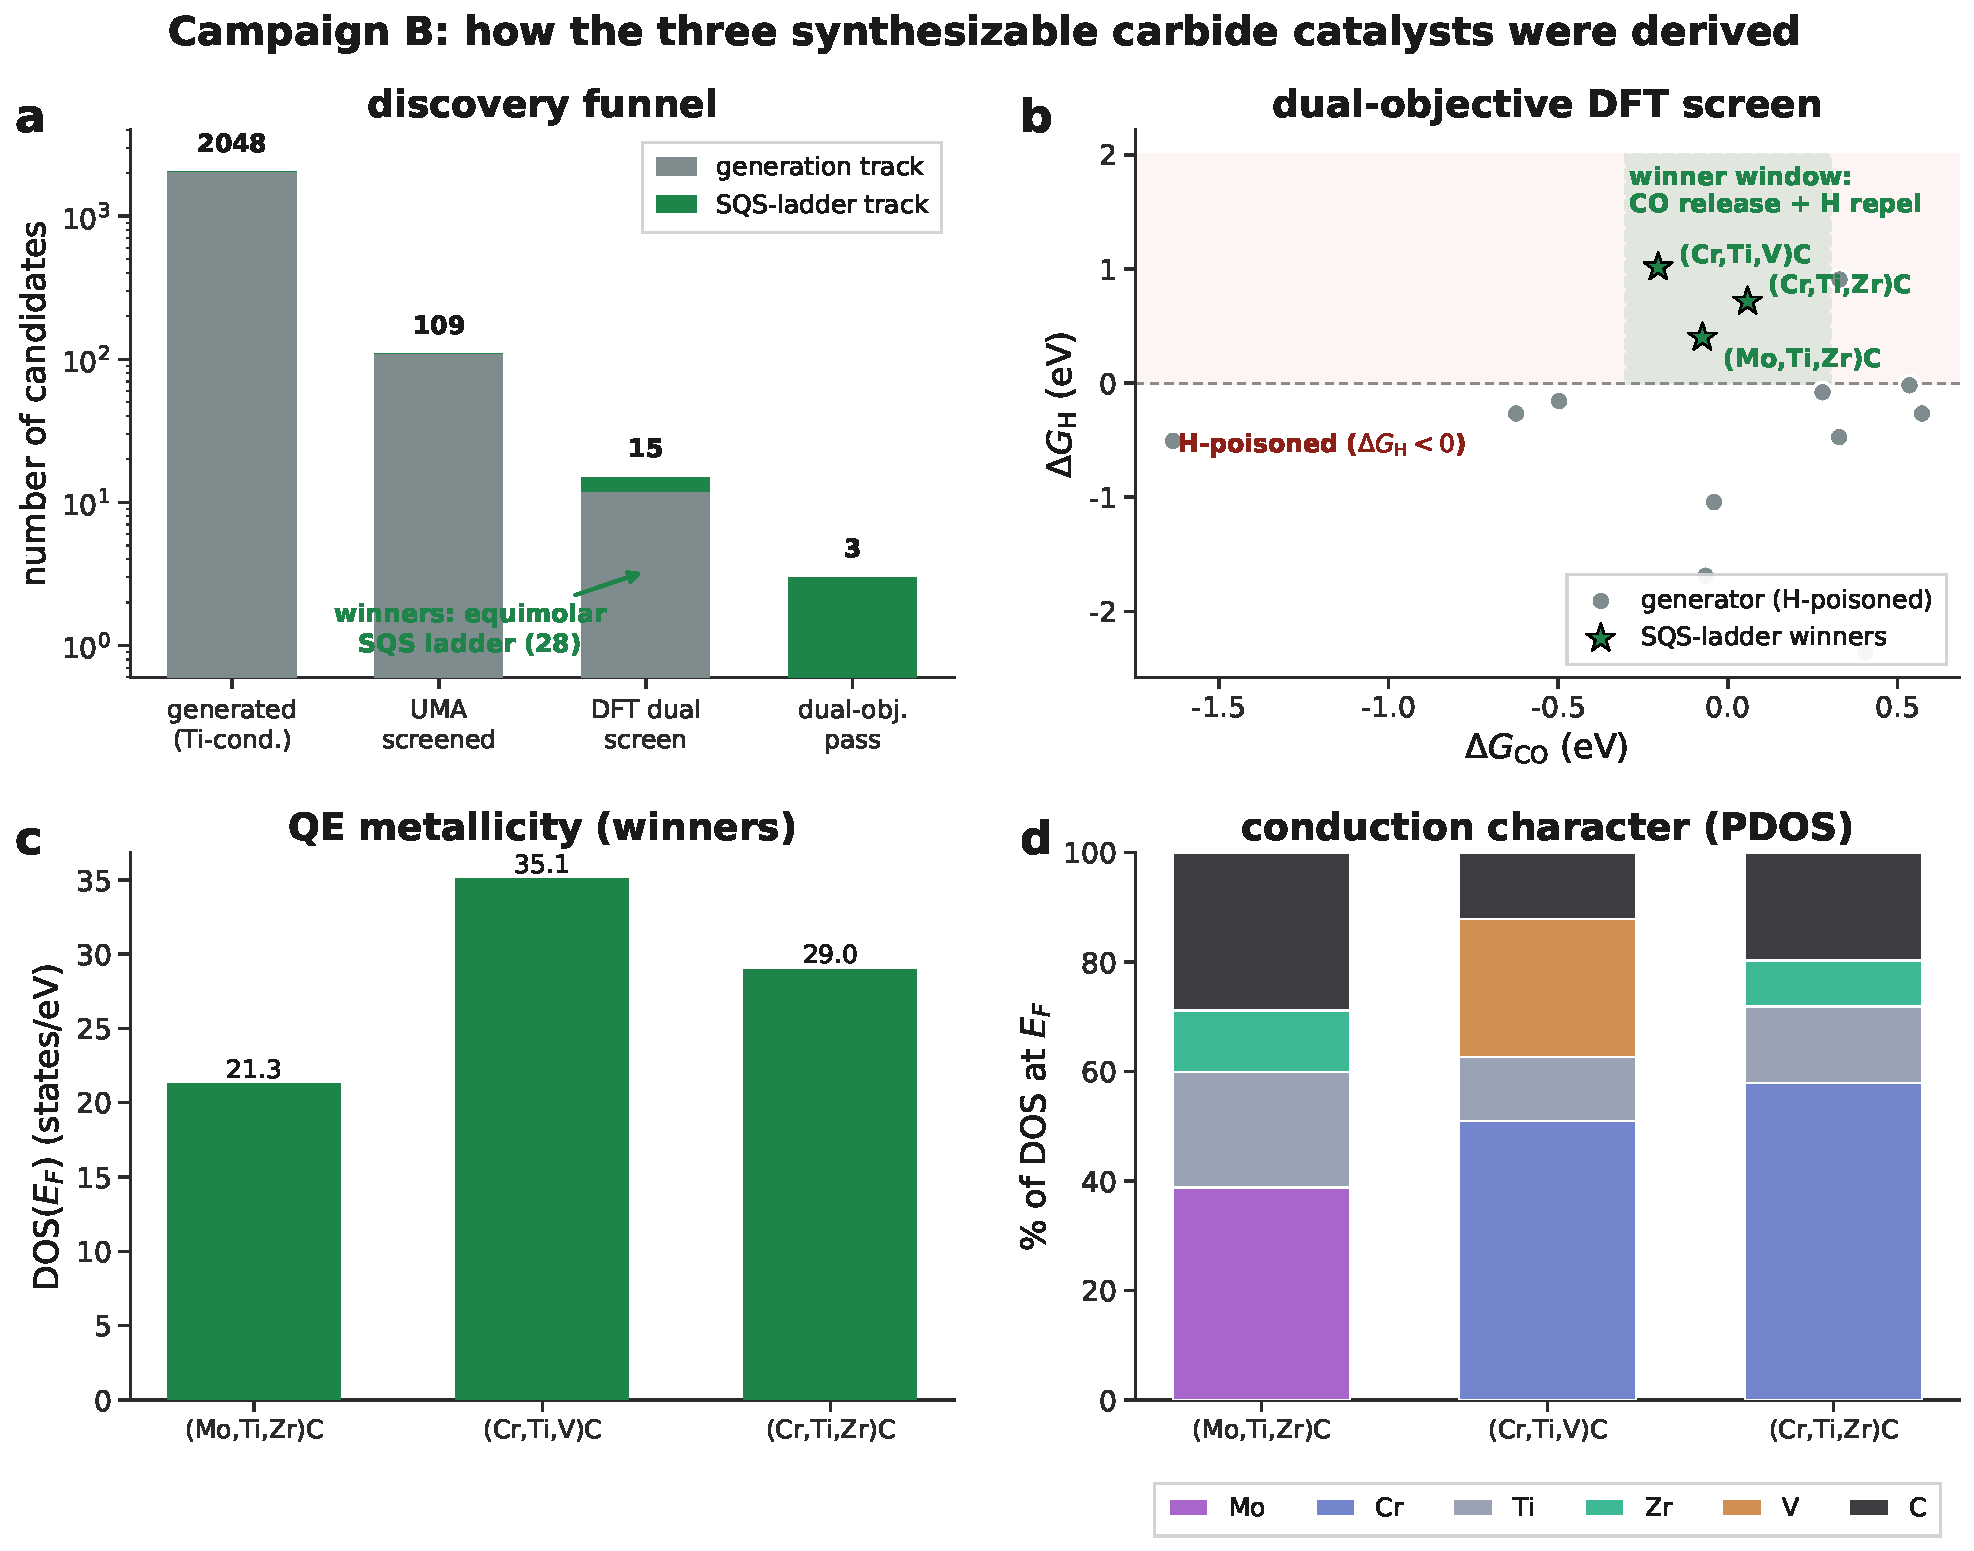
\includegraphics[width=\textwidth]{fig_co2rr_pipeline_summary_B.pdf}
\caption{캠페인 B 종단간 도출 종합 --- 그림~\ref{fig:summary}(캠페인 A)의 탄화물 대응.
(a) 발견 깔때기: Ti-조건화 생성 2048종 $\to$ UMA 스크린 $\to$ DFT 이중목표 스크린 15종 $\to$
이중목표 통과 3종. \emph{생성 트랙}(회색)은 DFT에 오른 12종이 \emph{모두} H-피독으로 탈락(0종 통과)한
반면, 3종의 승자는 \emph{등몰 SQS 사다리}(초록)에서 나왔다 --- 즉 생성 모형이 H-반발 Ti-rich 화학을
과소표집하여, 승자는 체계적 SQS 구성으로 확보되었다. (b) DFT 이중목표 스크린: $\dGCO$ 대 $\dGH$.
승자 창(CO 방출 $|\dGCO|<0.3$ \emph{그리고} H 반발 $\dGH>0$)에 Ti계 3종(별표)만 들며, 생성 후보
12종은 $\dGH<0$로 피독된다. (c) 3 승자의 QE 벌크 금속성 DOS($E_F$). (d) 원소 투영 전도 특성
($E_F$에서 원소별 DOS 비중). (c,d)는 캠페인 A의 그림~\ref{fig:summary}(c,d)와 동일 계산 수준(QE
벌크 SCF$\to$dos$\to$projwfc).}
\label{fig:summaryB}
\end{figure}

\paragraph{조성과 구조.} 세 후보는 모두 \emph{등몰 3금속 암염형 모노카바이드}
$(M,M',M'')\mathrm{C}$이며 금속:탄소 $=1:1$이다(표~\ref{tab:comp}): hec3-MoTiZr $=$
$(\mathrm{Mo},\mathrm{Ti},\mathrm{Zr})\mathrm{C}$, hec3-CrTiV $=(\mathrm{Cr},\mathrm{Ti},\mathrm{V})\mathrm{C}$,
hec3-CrTiZr $=(\mathrm{Cr},\mathrm{Ti},\mathrm{Zr})\mathrm{C}$. 64원자 SQS (100) 슬랩의 금속 카운트는
$11{:}11{:}10$으로 등몰을 근사한다(예: Mo$_{11}$Ti$_{11}$Zr$_{10}$C$_{32}$). 금속 부격자는 모두 산-침출
안정 4/5/6족 전이금속이므로 캠페인의 설계 제약(A3)을 만족한다.

\begin{table}[t]
\centering
\caption{캠페인 B 최종 후보의 조성·구조와 합성 가능성 지표. VEC는 금속 평균 원자가전자수(4/5/6족
$=4/5/6$). ``산-안정''은 산-침출 생존(A3). $E_{\mathrm{hull}}$(eV/atom)은 QE-PBE 생성에너지와 Materials
Project 볼록 껍질(GGA/GGA+U)로 계산: 세 후보 모두 캠페인 A(REE, $+0.15\!\sim\!+0.36$)보다 안정하며,
MoTiZr는 사실상 껍질 위($\approx\!0$)다.}
\label{tab:comp}
\setlength{\tabcolsep}{3pt}\footnotesize
\begin{tabular}{llcccccc}
\hline
후보 & \shortstack{이상\\조성} & \shortstack{슬랩\\(64원자)} & 구조 & \shortstack{활성\\면} & VEC & \shortstack{산-\\안정} & $E_{\mathrm{hull}}$ \\
\hline
hec3-MoTiZr & $(\mathrm{Mo,Ti,Zr})\mathrm{C}$ & Mo$_{11}$Ti$_{11}$Zr$_{10}$C$_{32}$ & 암염 $MC$ & (100) & 4.67 & $\bigcirc$ & $-0.02$ \\
hec3-CrTiV  & $(\mathrm{Cr,Ti,V})\mathrm{C}$  & Cr$_{11}$Ti$_{11}$V$_{10}$C$_{32}$  & 암염 $MC$ & (100) & 5.00 & $\bigcirc$ & $+0.05$ \\
hec3-CrTiZr & $(\mathrm{Cr,Ti,Zr})\mathrm{C}$ & Cr$_{11}$Ti$_{11}$Zr$_{10}$C$_{32}$ & 암염 $MC$ & (100) & 4.67 & $\bigcirc$ & $+0.10$ \\
\hline
\end{tabular}
\end{table}

\begin{table}[t]
\centering
\caption{캠페인 B 최종 후보의 DFT 활성점·자유에너지 요약. $\Delta G$ 단위 eV, $U_L$ 단위 V vs RHE.
활성면은 모두 (100); 셋 다 CO 발생($|\dGCO|<0.3$)과 H 반발($\dGH>0$)을 동시 만족한다. 전위 결정
단계(PDS)는 세 후보 모두 $*$COOH 형성($\mathrm{CO_2}\!+\!*\!\to\!{*}\mathrm{COOH}$)이다.}
\label{tab:dual}
\setlength{\tabcolsep}{4pt}\footnotesize
\begin{tabular}{llcccccl}
\hline
후보 & 방법 & $*$CO 활성 자리 & $\dGCO$ & $\dGCOOH$ & $\dGH$ & $U_L$ & 판정 \\
\hline
hec3-MoTiZr & 단일점 & Mo ontop(약결합) & $-0.08$ & $+0.13$ & $+0.40$ & $-0.13$ & CO 선택 \\
hec3-MoTiZr & \textbf{이완} & Mo ontop(방출) & $+0.18$ & $+0.39$ & $+0.57$ & $-0.40$ & \textbf{CO 선택(확인)} \\
hec3-CrTiV  & 단일점 & Cr ontop & $-0.20$ & $+0.73$ & $+1.01$ & $-0.73$ & CO 선택 \\
hec3-CrTiZr & 단일점 & Cr ontop & $+0.06$ & $+0.72$ & $+0.71$ & $-0.72$ & CO 선택 \\
\hline
\end{tabular}
\end{table}

\paragraph{활성 자리.} 이완/스크린 기하에서 흡착물의 최근접 금속(주기 최소상 거리)을 보면 뚜렷한
패턴이 있다: $*$CO는 세 후보 모두 \emph{6족 금속 ontop}에 결합한다(CrTiV의 Cr $\sim\!1.9$~\AA,
CrTiZr의 Cr $\sim\!2.0$~\AA, MoTiZr의 Mo $\sim\!2.1$~\AA). 다만 결합 세기가 달라, MoTiZr는 약결합
($\dGCO\!=\!+0.18\!>\!0$)이라 CO를 \emph{방출}하고 CrTiV는 강결합($\dGCO\!=\!-0.20$)이라 CO를
붙든다. $*$H는 금속 ontop/bridge에
앉되(예: MoTiZr는 Mo 위 $1.76$~\AA, CrTiZr는 Zr 브리지 $\sim\!2.1$~\AA) 자유에너지상 불리하여
피복이 억제된다. 즉 CO 결합은 6족 금속이, H 반발은 4족-rich(저 VEC) 골격이 각각 조율한다. 세
후보의 (100) 표면 CO 활성 사이트를 그림~\ref{fig:sites}에 도시하였다.

\begin{figure}[t]
\centering
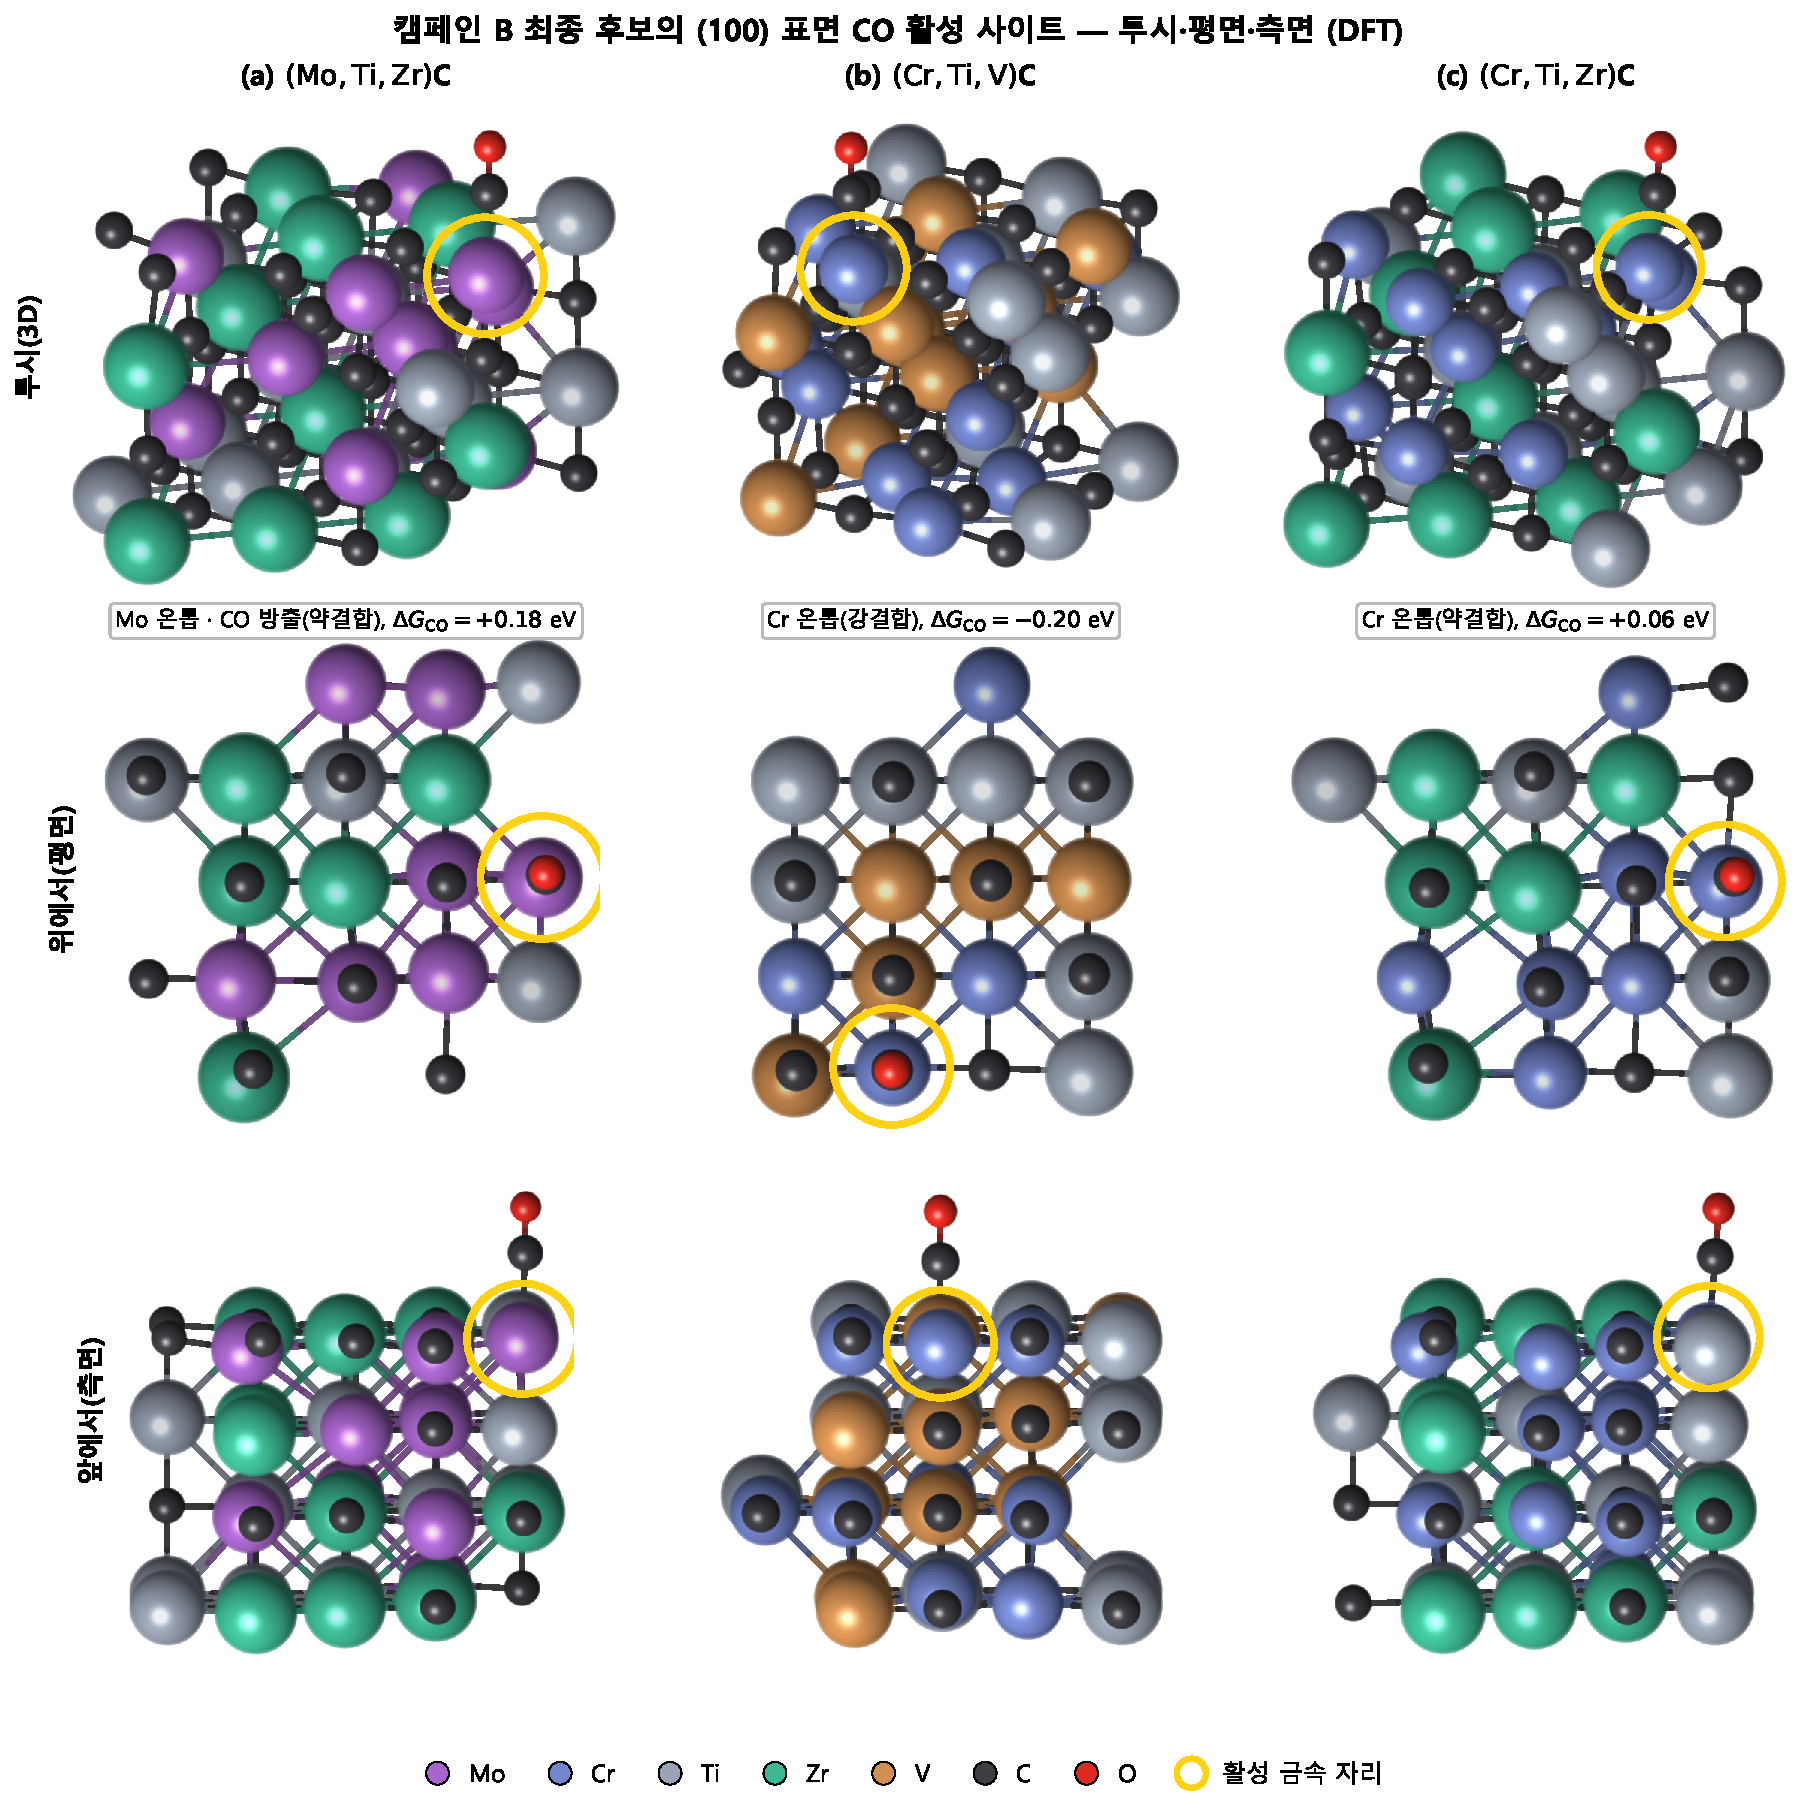
\includegraphics[width=\textwidth]{fig_co2rr_active_sites.pdf}
\caption{캠페인 B 세 최종 후보의 (100) 표면 CO 활성 사이트(DFT 이완/스크린 기하). \textbf{열}은 세
후보, \textbf{행}은 투시(3D)$\,\cdot\,$평면도(위에서 수직)$\,\cdot\,$측면도(앞에서)이며, 각 패널의
노란 링이 흡착 CO의 최근접(활성) 금속 자리다. 평면도는 활성점 바로 위에 CO 산소(빨강)가 겹쳐 보이고,
측면도는 CO가 표면에서 수직으로 올라선 \emph{ontop} 결합을 보여 활성 위치를 직관적으로 알 수 있다.
(a) $(\mathrm{Mo,Ti,Zr})$C는 CO가 \emph{Mo ontop}에 약하게 결합하나($\sim\!2.1$~\AA)
$\dGCO\!=\!+0.18\!>\!0$이라 \emph{방출}된다(이완). (b) $(\mathrm{Cr,Ti,V})$C와
(c) $(\mathrm{Cr,Ti,Zr})$C는 CO가 \emph{Cr ontop} 자리에 결합한다($\sim\!1.9$--$2.0$~\AA).
세 후보 모두 CO 결합/방출은 6족(Cr/Mo) 자리가 조율한다. 원자색은 범례 참조; 활성면은 모두 (100).}
\label{fig:sites}
\end{figure}

\paragraph{자유에너지 다이어그램: HER 억제, CO$_2$RR 선호.} 세 후보의 CO$_2$RR(CO$_2\!\to\!$CO)와
HER 자유에너지 다이어그램을 그림~\ref{fig:cheher}에 함께 제시한다. CO$_2$RR 경로는 인가 한계 전위
$U_L$에서 접근 가능한 반면, HER 중간체 $*$H는 세 후보 모두 자유에너지상 \emph{양(+)}으로 솟아 있어
($\dGH\!=\!+0.57\!\sim\!+1.01$~eV) H 피복이 억제된다 --- 즉 \emph{동일한 표면이 HER을 억제하면서
CO$_2$RR을 선호}한다. 다만 CO는 \emph{관문 중간체}이며, 그 너머 에탄올 등 다중탄소(C$_{2+}$)로의 심화
환원은 C--C 짝지음 경로(\ref{sec:tandem}절)의 계산이 필요하므로 여기서는 개념적으로(회색 점선)만
표시한다 --- 완전한 CO$_2\!\to\!$에탄올 다이어그램은 향후 과제다(기존 CO$_2\!\to\!$CO 다이어그램,
\ref{fig:che}도 같은 이유로 CO에서 멈춘다).

\begin{figure}[t]
\centering
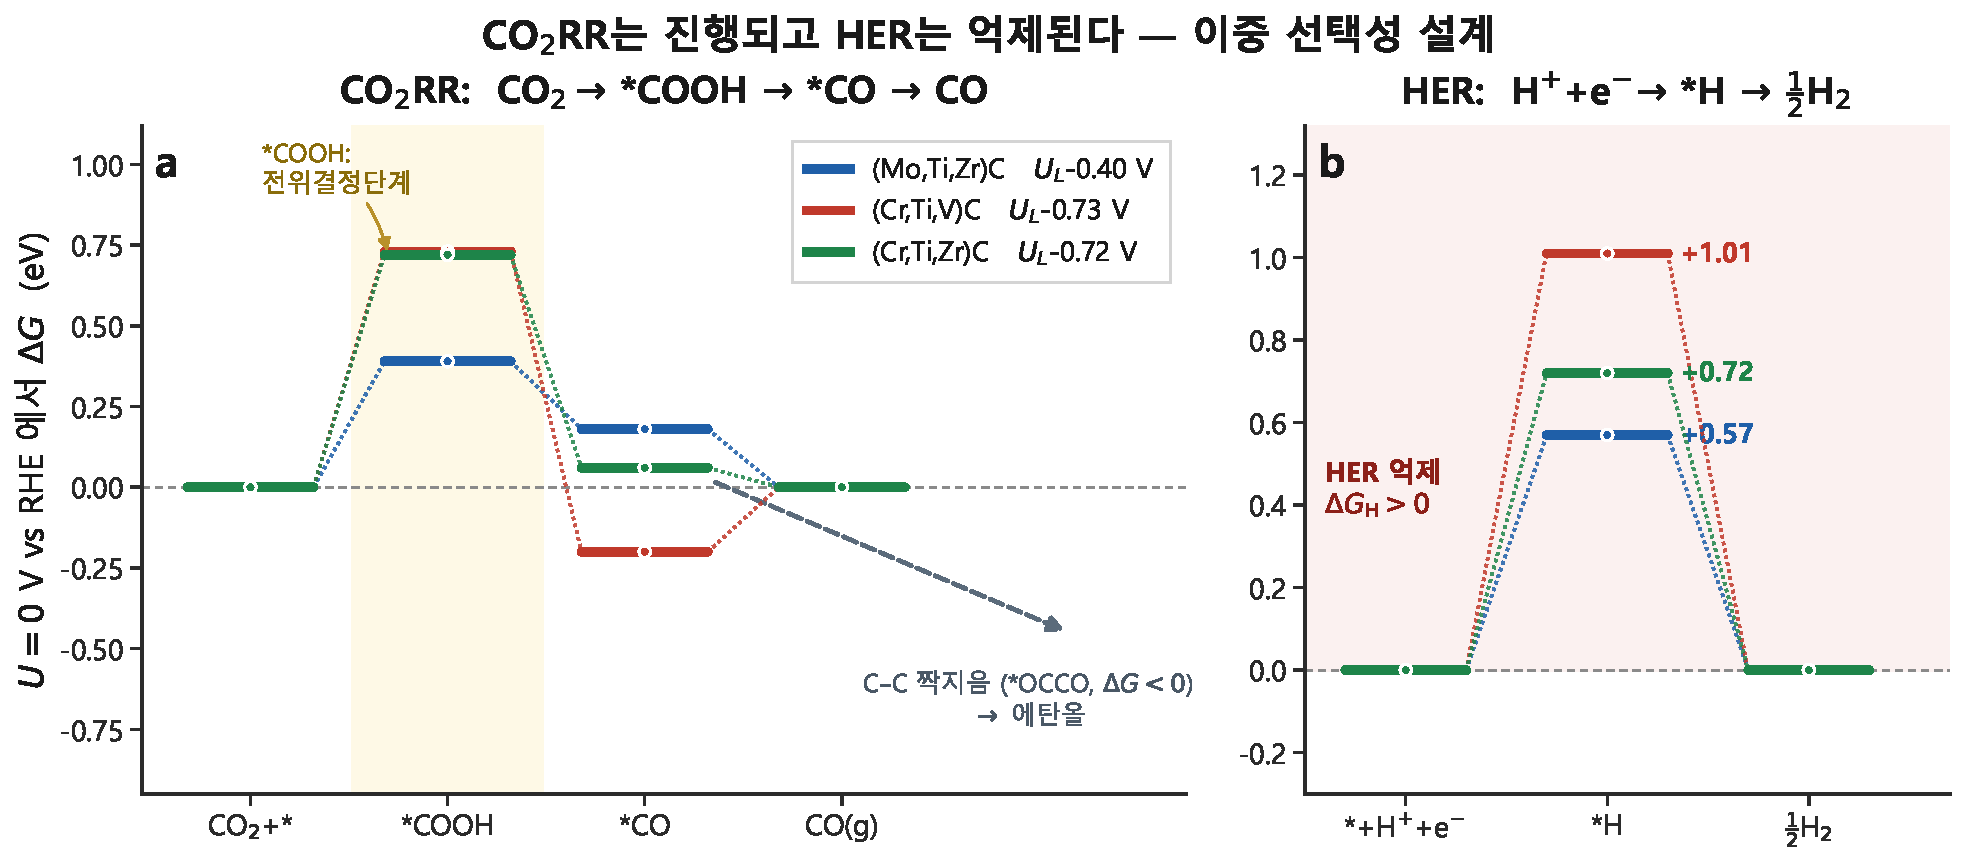
\includegraphics[width=\textwidth]{fig_co2rr_che_her.pdf}
\caption{캠페인 B 세 최종 후보의 자유에너지 다이어그램($U=0$ vs RHE). (a) CO$_2$RR:
CO$_2\!\to\!*$COOH$\!\to\!*$CO$\!\to\!$CO; 전위 결정 단계는 세 후보 모두 $*$COOH 형성이다. $*$CO 이후
에탄올(C$_{2+}$)로의 경로: C--C 짝지음 첫 중간체($*$OCCO, C--C$\approx$1.5~\AA, $\Delta G<0$)를 계산해
C2(에탄올) 경로가 유리함을 확인하였고(C1 $*$CHO는 흡열; \ref{sec:tandem}절), 회색 점선은 그 이후
전체 경로가 아직 개념(전이상태·완전 경로 미계산)임을 뜻한다.
(b) HER: H$^+\!+\!$e$^-\!\to\!*$H$\!\to\!\tfrac12$H$_2$; $*$H 준위가 세 후보 모두 양($\dGH>0$)이어서
HER이 억제된다(음영 영역). 두 패널의 $y$축 상단 스케일을 맞추어 CO$_2$RR의 율속 준위($*$COOH)와 HER의
$*$H 높이를 직접 비교할 수 있다. hec3-MoTiZr는 이완값, 나머지는 단일점.}
\label{fig:cheher}
\end{figure}

\paragraph{대표 후보의 완전 이완: 선택성은 견고, 한계 전위는 정정.} 헤드라인 후보 hec3-MoTiZr의
활성 (100) 면에 대해 청정슬랩·$*$CO·$*$COOH·$*$H를 완전 이온 이완(GPU QE, 하부 절반 고정,
$\Gamma$)하였다. \ref{sec:stagec}절과 같은 이유로 무대칭 64원자급 슬랩은 16~GB VRAM에서
$2{\times}2{\times}1$ $k$-메시가 16.4~GB로 실행 불가하여 $\Gamma$로 이완하였고, $\Delta G$가 동일
셀 차분이라 유한-$k$ 오차가 상쇄됨은 앞서 검증하였다. \textbf{핵심 선택성 주장은 이완에도 견고}하다:
$\dGH=+0.57$~eV로 오히려 단일점($+0.40$)보다 \emph{강화}되어 H 반발이 기하 인공산물이 아님을 확인하며,
$\dGCO=+0.18$~eV로 CO는 여전히 약결합·탈리한다(CO 선택적=YES). 반면 \textbf{한계 전위는 정정}된다:
이완 시 $*$COOH 형성($\dGCOOH=+0.39$~eV)이 흡열이 되어 전위 결정 단계가 되고
$U_L=-0.40$~V(단일점 $-0.13$)로 악화된다. 즉 완전 이완은 \emph{선택성을 확증}하되 \emph{겉보기 활성을
정정}하여, 단일점 DFT$/\!/$UMA가 $*$COOH 장벽을 과소평가했음을 드러낸다 --- 이완 검증의 가치를
그대로 보인다. 이완된 최종 구조(그림~\ref{fig:moTiZr})는 이중 선택성을 기하로 직접 보여준다:
$*$CO는 이완 후에도 Mo \emph{ontop}에 약하게 결합($\sim\!2.1$~\AA)하나 $\dGCO\!=\!+0.18\!>\!0$이라
열역학적으로 \emph{방출}되어 표면을 피독하지 않고, $*$H는 표면에 흡착하되($\sim\!1.7$~\AA)
자유에너지상 불리하여($\dGH\!=\!+0.57$~eV) 피복률이 낮게 유지된다.

\begin{figure}[t]
\centering
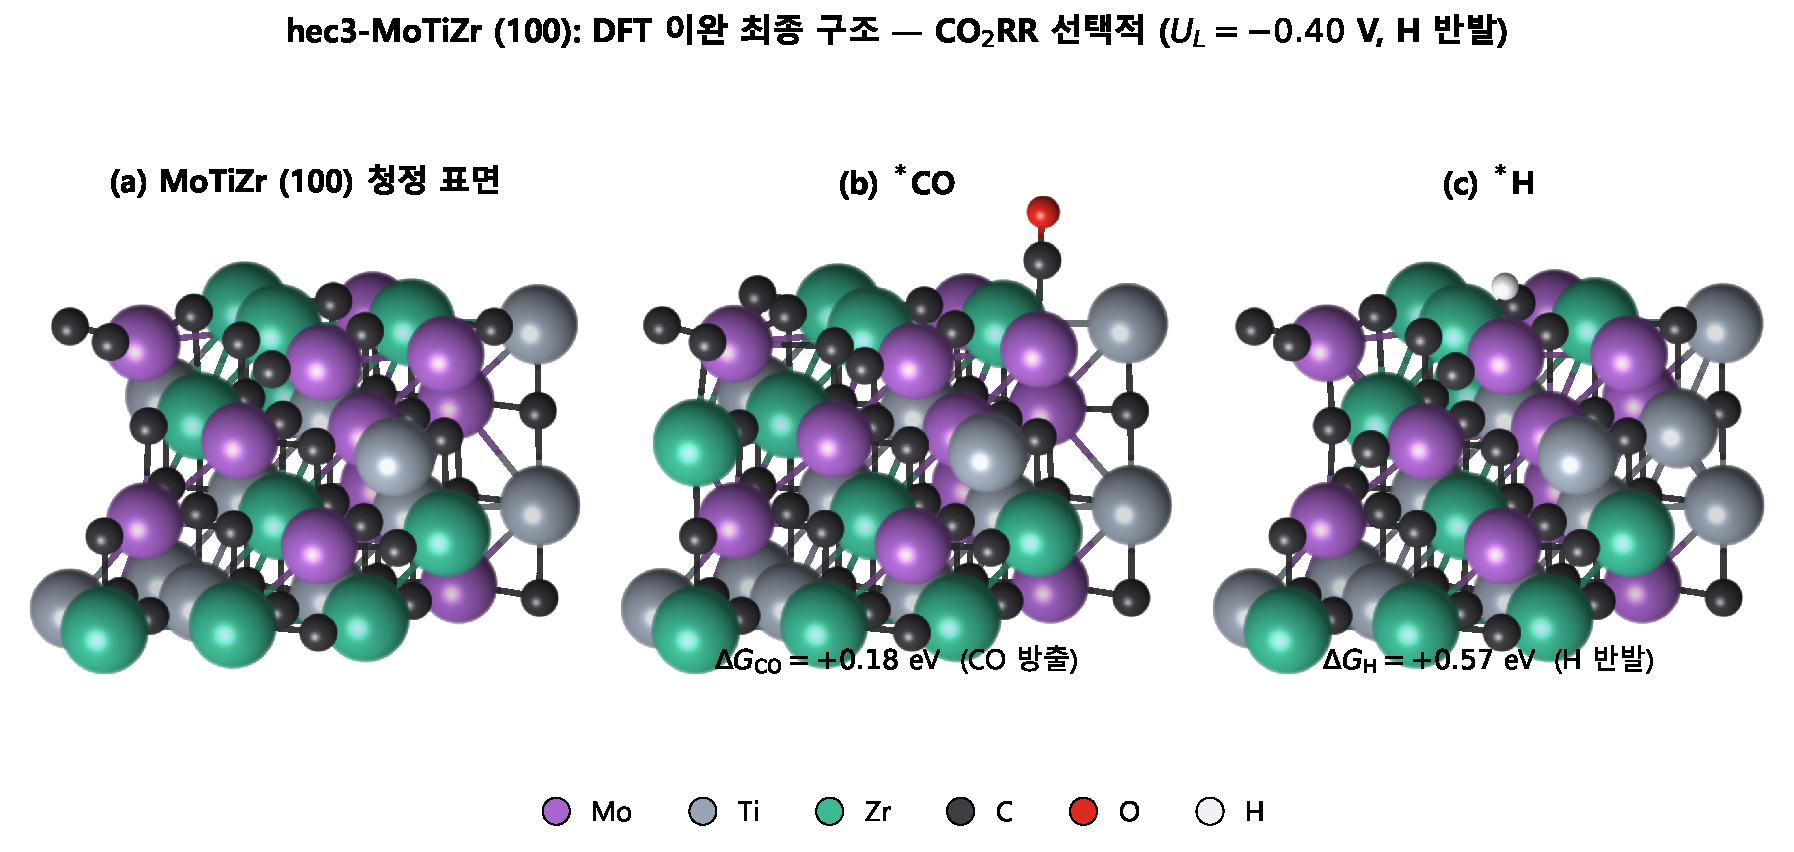
\includegraphics[width=\textwidth]{fig_co2rr_moTiZr_structure.pdf}
\caption{헤드라인 후보 \textbf{hec3-MoTiZr (100)}의 DFT 완전 이완 최종 구조(SQS 64원자 슬랩,
하부 절반 고정, $\Gamma$). (a) 청정 표면, (b) $*$CO, (c) $*$H. 이중목표가 기하로 드러난다:
$*$CO는 이완 후에도 Mo ontop에 약하게 결합($\sim\!2.1$~\AA)하나 $\dGCO=+0.18\!>\!0$이라
\emph{방출}되고, $*$H는 표면에 흡착하나 자유에너지상 불리하여($\dGH=+0.57$~eV, H 반발) 피복이 억제된다. 즉 표면은
CO$_2$RR 중간체 자리를 비워 두면서 HER을 억제한다($U_L=-0.40$~V vs RHE, CO$_2$RR 선택적).
원자색: Mo 보라, Ti 회색, Zr 녹색, C 진회색, O 적색, H 백색. 좌표 파일은
\texttt{results\_cif/MoTiZr\_*.cif}.}
\label{fig:moTiZr}
\end{figure}

\paragraph{생성 모형의 재조준: 저-VEC 조건화가 발견을 이끈다.} 위 3승자는 고엔트로피 SQS
사다리(\ref{sec:outstanding}절)에서 나왔고 생성 모형 직접 산물은 아니었다 --- 초기 CO-조건화가
Nb/Ta/Mo-rich(H 피독) 조성으로 치우쳤기 때문이다. 이에 조건화를 \emph{저 VEC(4.5)}로 재조준해
2048개를 재생성한 결과, \textbf{생성 모형 자체가 이중목표 승자}를 산출하였다(UMA 면별 스크린 기준
3종: HfZrTa$_2$Nb-C~(110) $\dGCO\!=\!-0.06$/$\dGH\!=\!+0.22$, HfTaNb-C~(011) $-0.10$/$+0.21$,
HfZr$_3$TaNb-C~(011) $-0.13$/$+0.18$; 모두 4/5족-rich 저 VEC). 반발 여유는 SQS 승자($\dGH\!=\!+0.4\!\sim\!+1.0$)보다
작지만, \emph{이전에는 SQS 사다리에서만 나오던 H-반발·CO-발생 표면을 이제 생성 모형이 직접 제안}한다는
점이 핵심이며, VEC 레버의 인과적 유효성을 확인한다.

\paragraph{정직한 유의점.} (i) 확정 3승자는 명시적 SQS 고용체이지 생성 산물이 아니다(위 재조준으로
생성 산물 승자를 별도 확인). (ii) hec3-CrTiV/CrTiZr는 단일점(DFT$/\!/$UMA)이며, 다만 H-반발 여유가
커($\dGH\!=\!+1.01$/$+0.71$) 이완 민감도가 대표 후보보다 낮다. (iii) 대표 후보 이완은 $\Gamma$ 수준의
국소 이완(느슨한 힘 수렴 0.26~eV/\AA)으로, 단일점보다 낫되 $k$-수렴은 아니다 --- 이완 중 관찰된
$\sim$0.5~eV 기하 이동 자체가 단일점의 이 한계를 방증한다. (iv) 등몰 SQS 이상화이며, \emph{순서화된}
소형 대리셀은 이 이중 거동을 재현하지 못한다(순서화 시 CO 발생면과 H 반발면이 분리됨) --- 즉 이중
활성은 \emph{무질서·조성 특유}의 성질이다. (v) $\dGCO\!\approx\!0$은 C--C 짝지음이 아니라 \emph{CO
공급원}을 뜻하며, 에탄올 등 C$_{2+}$ 목표에는 CO를 방출하는 본 카바이드와 짝짓는 별도 커플러가 필요하다.

% =====================================================================
\chapter{계획된 실험 검증}
\label{ch:experiment}

\noindent 실험 검증은 \emph{제조 가능한} 캠페인 B 최종 후보(hec3-MoTiZr를 대표로, CrTiV/CrTiZr 포함)를
대상으로 한다 --- 캠페인 A의 희토류 후보는 산-침출에서 용해되어 애초에 시험 대상이 될 수 없으며, 바로
그 제약이 캠페인 B의 산-안정 전이금속 팔레트를 규정하였다(\ref{sec:campaignB}절). 파이프라인은 구체적이고
반증 가능한 예측을 제시한다: 이들 후보는 (i) 단일상 금속성 카바이드로 합성 가능하고 (ii) HER을 능가하는
선택성으로 이산화탄소를 일산화탄소로 전기환원해야 한다. 본 장은 이를 시험하기 위해 설계된 실험 프로그램을
명시한다. 결과는 캠페인 완료 시 보고한다.

\section{소재 합성}
캠페인 B 최종 후보(Ti 기반 전이금속 카바이드)는 볼밀링된 금속/산화물 전구체의 고온 탄화(또는 아크
용융 후 탄화)로 합성하여 SQS 예측의 거의 등몰 금속 부격자를 목표로 한다. 금속열환원--산-침출 경로를
쓰는 경우에도 이 조성은 침출 단계를 견딘다(산-안정 팔레트로 설계된 결과). 상 순도와 단일상 암염형/육방정 구조는
분말 X선 회절(XRD)로, 금속 분포의 균질성은 SEM/EDS 및 STEM-EDS 매핑으로, 표면 조성/산화 상태는
X선 광전자 분광법(XPS)으로 검증한다. \tbu{합성 및 구조 분석}

\section{전기화학 CO\texorpdfstring{$_2$}{2}RR 시험}
촉매 잉크를 기체확산 또는 유리질 탄소 전극에 드롭캐스트하고, CO\textsubscript{2} 포화 수용성
중탄산염 전해질에서 기밀 H-셀(및 높은 전류밀도를 위한 MEA/흐름 셀)로 시험한다. 일련의 인가
전위에서의 선형 주사 전압전류법과 정전위법으로 부분 전류밀도를 정량화하며, 기하학적 및 전기화학적
활성 표면적으로 규격화한 활성을 보고한다. \tbu{분극 곡선 및 전위별 패러데이 효율}

\section{생성물 분석}
\begin{itemize}[nosep]
\item \textbf{기체 생성물(CO, H\textsubscript{2}, 잔류 CO\textsubscript{2}).} 셀 헤드스페이스/출구를
가스 크로마토그래프(TCD + 메탄화기 부착 FID)로 온라인 샘플링하여 CO와 H\textsubscript{2}를 정량하고
이로부터 CO 패러데이 효율과 CO/H\textsubscript{2} 선택성을 산출하며, CO\textsubscript{2} 전환율은
입구/출구 물질수지로 추적한다. 온라인 미분 전기화학 질량분석(DEMS)으로 전위 분해된 CO/H\textsubscript{2}
개시를 제공한다. \tbu{GC/DEMS 기체 생성물 정량}
\item \textbf{액상 생성물.} 음극액은 물 억제와 내부 표준(예: DMSO/DSS)을 적용한 정량
\textsuperscript{1}H 핵자기공명(NMR) 분광법으로 분석한다. \emph{예비 전기분해에서 에탄올이
\textsuperscript{1}H NMR로 검출}되었으며(폼산 등 여타 액상 생성물과 함께), 이는 설계가 겨냥한
2전자 CO 경로를 \emph{넘어} 다중탄소(C\textsubscript{2+}) 생성이 실제로 일어남을 보인다. 이 관찰은
고엔트로피 표면의 자리 다양성이 CO 생성과 C--C 짝지음을 한 물질에서 매개하는 \emph{다중 자리
탠덤}으로 해석된다(\ref{sec:tandem}절). 각 액상 생성물의 농도·패러데이 효율 정량과 에탄올 대 CO
분배는 \tbu{\textsuperscript{1}H NMR 액상 생성물 정량(에탄올 FE 포함)}
\item \textbf{흡착 중간체.} In-situ 감쇠 전반사 표면증강 적외선 흡수 분광법(ATR-SEIRAS / FT-IR)으로
전위에 따른 *COOH 및 선형/브리지 결합 *CO 밴드를 검출하여, 계산된 $\dGCOOH$ 및 $\dGCO$ 디스크립터와
직접적인 메커니즘적 연결을 제공한다. \tbu{*COOH/*CO 중간체의 in-situ FT-IR}
\end{itemize}

\section{안정성 및 사후 분석}
장시간 전기분해로 내구성을 평가하고, 시험 전후의 XRD, XPS, 현미경으로 표면 산화, 희토류 성분의 용출,
카바이드 네트워크 무결성을 조사한다. \tbu{내구성 및 사후 특성 분석}

\section{검증 논리}
실험은 전산 예측을 항목별로 시험하도록 설계된다: 금속 전도성(4단자 탐침/전기화학 임피던스)을 DFT DOS와,
CO 선택성(GC/NMR)을 계산된 $\dGCO$ 및 $\dGCOOH<\dGH$ 선택성 기준과, 메커니즘 중간체(FT-IR)를
디스크립터 사다리와 대조한다. 예측-측정 비교표는 완료 시 보고한다(표~\ref{tab:expt}).

\begin{table}[t]
\centering
\caption{전산 예측과 실험 관측량의 계획된 비교.}
\label{tab:expt}
\small
\begin{tabular}{lll}
\toprule
예측 (본 연구) & 실험적 검증 수단 & 상태\\
\midrule
단일상 HEC, 등몰 금속 & XRD, STEM-EDS & \tbu{결과}\\
금속성($\Ef$에서 유한 DOS) & 4단자/EIS & \tbu{결과}\\
CO 선택성, $\dGCOOH<\dGH$ & GC, \textsuperscript{1}H NMR, FE & \tbu{결과}\\
*COOH$\rightarrow$*CO 경로 & in-situ FT-IR & \tbu{결과}\\
CO\textsubscript{2} 전환율 & 입출구 GC 수지 & \tbu{결과}\\
\bottomrule
\end{tabular}
\end{table}

% =====================================================================
\chapter{고찰}
\label{ch:discussion}

\section{이 파이프라인을 채택한 이유와 그 이점}
본 논문의 핵심 방법론적 주장은 \emph{경제성 제약이 생성 단계에 속한다}는 것이다. 확산 모델을 고가
금속 분율 라벨로 미세조정하고 0으로 유도함으로써, 저렴한 부분공간이 \emph{구성적으로} 표본
추출되며, 이는 그것이 희소한 무제약 후보군을 필터링하여 발견하는 방식과 대비된다. 그 결과 깔때기는
$\sim$10\textsuperscript{3}개 후보를 조사하면서도 DFT는 6개 구조에만 사용하며, 각 단계(조성 대리지표
$\rightarrow$ MLIP $\rightarrow$ DFT)는 이전 단계가 이미 탐색 공간의 대부분을 제거한 곳에 정확도를
더한다. 이는 일반화 가능한 틀이다: 조건화 디스크립터를 교체하면 동일한 기계가 다른 반응으로 재조준된다.

\section{후보의 해석}
아래는 \emph{캠페인 A}(활성-우선 기준선)의 여섯 후보에 대한 해석으로, 파이프라인이 유효한 활성·전도
디스크립터 영역을 포착함을 보인다. 다만 이들은 제조 가능성 관문에서 탈락하므로(\ref{sec:ree-stability}절),
\emph{제조 가능한} 최종 촉매는 캠페인 B의 Ti 기반 카바이드(대표 hec3-MoTiZr, \ref{sec:campaignB}절)이다.
여섯 후보 모두 저렴한 초기 전이금속(Y, Zr, W)을 경희토류(La, Ce, Pr)와 카바이드 금속 부격자 위에서
결합한다. DFT로 규명한 전도 특성(그림~\ref{fig:pdos})은 탄소 $2p$ 네트워크 금속에서 금속 $d$ 금속까지의
연속을 보이며, 이는 탄소가 금속 $d$ 상태를 재구성하는 ``백금 유사'' 그림~\cite{levy1973}을 반영한다.
거의 열중성인 $\dGCO$와 $\dGCOOH<\dGH$ 선택성은 이들 소재를 Au/Ag/Zn을 CO 선택적으로 만드는 동일한
디스크립터 영역에 위치시키되~\cite{hori2008}, 지구상에 풍부한 구성원소로 구현한다---이것이 바로 설계
목표이다. 고엔트로피 합금이 실험적 CO\textsubscript{2}/CO 환원 촉매로 성공한 점~\cite{nellaiappan2020,batchelor2019}과
Mo\textsubscript{2}C가 선택적 CO\textsubscript{2}-to-CO에 성공한 점~\cite{porosoff2014}은 카바이드+HEC
경로의 외적 타당성을 뒷받침한다.

\section{표면 산화·OH 피독: 잠정 결론과 조성 처방}
\label{sec:disc-poison}
희토류의 큰 산소친화도 때문에 ``수용액에서 산화되어 활성점을 덮지 않는가''는 이 소재군의 핵심
우려다. 이를 같은-면 완전 표면 Pourbaix($*$CO/$*$COOH/$*$H/$*$OH/$*$O, \ref{sec:ree-stability}절)로
검토한 결과를 잠정 결론으로 정리한다.

\paragraph{작동 조건에서는 산화 피독이 아니다.} 각 후보의 활성 면에서 반응 중간체 $*$COOH를 포함해
정지상태를 판정하면, \textbf{작동 전위($-0.3\!\sim\!-1.0$~V vs RHE)에서 여섯 후보 모두 $*$COOH(작동
상태)가 우세}하며 $*$O/$*$OH가 지배하지 않는다. 산화 피복은 개회로 부근($\sim\!0$~V)의 과도 상태에
국한된다. 즉 위험의 무대는 \emph{정상 작동}이 아니라 \emph{기동/개회로 및 공기·수분 노출}이다.

\paragraph{문제가 되는 조성: La-부화(富化) 조성.} 산화 \emph{경향}(최악 면 $*$OH 결합 세기)은
조성의 La 함량과 강하게 연동된다(표~\ref{tab:poison}). \textbf{La$_5$Y$_4$W$_2$C$_9$}(금속 부격자 La
45\%)는 $\Delta G_{*\mathrm{OH}}=-6.7$~eV로 압도적으로 깊어 개회로 산화·용출 위험이 가장 크며,
계산상으로도 GPU SCF가 수렴하지 않은 유일한 조성이었다. \textbf{La$_3$Y$_5$(WC$_3$)$_3$}는 활성 면에서
작동 상태에 도달하는 데 가장 큰 음극 바이어스($-0.6$~V)를 요구한다. 반면 La을 포함하지 않는 Ce/Pr/Y
기반 조성(CeY$_2$ZrWC$_7$, Pr$_3$Y$_2$WC$_6$ 등)은 $*$OH 결합이 온건하고($-3$~eV대 이하) 더 완만한
전위에서 작동 상태로 전환된다. 표준 환원 전위 역시 La($-2.38$~V)가 Ce/Pr보다 음이어서, \emph{La이
산화·용출의 주된 위험 원소}라는 그림과 일치한다.

\begin{table}[t]
\centering
\caption{조성별 La 함량과 산화 경향($*$OH 결합). 최악 면 $\Delta G_{*\mathrm{OH}}$가 깊을수록 개회로
산화 위험이 크다. 활성 면 값은 실제 반응 면에서 훨씬 약함(덜 산화적)을 보인다. 단위 eV.}
\label{tab:poison}
\small
\begin{tabular}{lccc}
\hline
후보 & 금속 중 La\% & 최악 면 $\Delta G_{*\mathrm{OH}}$ & 활성 면 $\Delta G_{*\mathrm{OH}}$ \\
\hline
La$_5$Y$_4$W$_2$C$_9$ & 45 & $-6.67$ & $-0.85$ \\
La$_3$Y$_5$(WC$_3$)$_3$ & 27 & $-2.41$ & $-1.04$ \\
Ce$_2$Y$_2$ZrWC$_6$ & 0 & $-3.85$ & $-1.57$ \\
CeY$_2$ZrWC$_7$ & 0 & $-3.39$ & $-0.80$ \\
Pr$_3$Y$_2$WC$_6$ & 0 & $-3.09$ & $-1.04$ \\
Y$_2$ZrWC$_8$ & 0 & $-3.30$ & $-1.13$ \\
\hline
\end{tabular}
\end{table}

\paragraph{해결 방향(처방).} (1) \emph{조성 설계}: La 함량(넓게는 산화 위험 큰 REE 분율)을 억제하도록
생성기를 유도한다. 본 파이프라인의 핵심 기법을 그대로 재사용하여, 경제성(비싼 금속 분율)을 조건화한
것과 동일하게 \textbf{표면 $*$OH 결합(또는 산화막 형성) 디스크립터를 열 번째 조건화 속성으로 추가}해
저산화성 부분공간을 구성적으로 표본추출한다. 활성($\Delta G_{\rm CO}\!\approx\!0$)과 내산화성(약한
$*$OH)을 \emph{공동} 조건화하면 CeY$_2$ZrWC$_7$형(저과전위+저산화성) 후보가 우선된다.
(2) \emph{운전 프로토콜}: 작동 전위에서 $*$COOH가 우세하므로, 개회로 체류를 최소화하고 신속히 음극
바이어스를 인가하며, 합성·이송을 공기·수분 차단 하에 수행한다. (3) \emph{동역학적 보호}: 벌크가 준안정
(\ref{sec:hull}절, 껍질 위 $+0.15\!\sim\!0.36$~eV/atom)이고 La의 용출 구동력이 크므로, 표면 부동태화
막이나 보호층으로 기동 산화를 억제하는 전략이 유효할 수 있다. 이 처방들은 \ref{ch:experiment}장의
XPS(표면 산화 상태)·ICP-MS(용출)·in-situ FT-IR($*$COOH/$*$CO 밴드)로 직접 검증한다.

\paragraph{잠정성.} 위 결론은 (i) 최악 면은 최악 경계이고 실제 유효 피복률은 미정량, (ii) 약결합
$*$OH에서 MLIP--DFT 일치가 낮으며($r{=}0.74$) DFT가 더 약한 결합을 주는 점, (iii) 벌크 Pourbaix 수치
도표가 미완인 점에서 잠정적이며, 실험이 최종 심판자다.

\section{캠페인 B 후보의 합성 가능성 평가}
\label{sec:synth-feasibility}
세 최종 후보(표~\ref{tab:comp})는 모두 등몰 3금속 암염형 모노카바이드 $(M,M',M'')$C이다. 실제 합성
가능성은 다음 요인들로 평가된다.

\paragraph{긍정 요인.} (i) \emph{산-침출 안정성(A3, 설계로 충족).} 금속 부격자가 전부 4/5/6족 전이금속
(Ti, Zr, V, Cr, Mo)이므로, 금속열환원--산-침출 경로의 침출 단계에서 희토류와 달리 용해되지 않는다
--- 이 제약이 애초에 팔레트를 규정하였다(\ref{sec:campaignB}절). (ii) \emph{구조적 선례.} 등몰 다금속
암염형 카바이드는 합성된 소재 계열이며, 내화성 5금속 암염 고엔트로피 카바이드가 엔트로피 디스크립터로
발견·합성된 바 있다~\cite{sarker2018}; 3금속 조성은 그보다 접근이 용이하다. (iii) \emph{안정 이성분
골격.} 구성 이성분 중 TiC·ZrC·VC는 열역학적으로 안정한 암염형이어서 골격을 안정화한다.

\paragraph{볼록 껍질 안정성(계산).} 캠페인 A와 \emph{동일한} 방식(QE-PBE 생성에너지 + Materials
Project GGA/GGA+U 볼록 껍질)으로 3종의 껍질 위 에너지 $E_{\mathrm{hull}}$을 계산하였다(표~\ref{tab:comp}):
\textbf{hec3-MoTiZr $\approx\!-0.02$(사실상 껍질 위, 안정), hec3-CrTiV $+0.05$, hec3-CrTiZr $+0.10$~eV/atom}.
세 후보 모두 캠페인 A의 REE 카바이드($+0.15\!\sim\!+0.36$, \ref{sec:hull}절)보다 \emph{안정}하며, 특히
MoTiZr는 볼록 껍질 위에 놓인다. MP가 예측하는 분해 경쟁상은 안정 이성분 카바이드(TiC, ZrC,
Mo$_2$C, Cr$_3$C$_2$, V$_6$C$_5$)이고 준안정 여유는 $\le\!+0.10$~eV/atom에 불과하여, 배열 엔트로피
안정화로 충분히 도달 가능한 범위다. 즉 캠페인 B 후보는 ``제조 경로가 확보된(산-안정) 데다 열역학적으로도
껍질 위\,--\,저준안정''이며, 캠페인 A의 제조 불가 REE 후보와 질적으로 다르다.

\paragraph{잔여 위험 요인.} (i) CrC와 $\delta$-MoC의 암염형은 순수상에서 준안정(또는 고압상)이므로
이들을 포함한 고용체는 \emph{배열 엔트로피 안정화}에 의존하나, 위 $E_{\mathrm{hull}}(\le\!+0.10)$이 그
여유가 작음을 정량 확인한다. (ii) QE(SSSP)와 MP(VASP) 참조 차이로 $\sim\!0.1$~eV/atom의 방법론적
불확실성이 있고(원소 상쇄로 대부분 소거되나 잔차 존재), Cr은 비자성 근사이며, MoTiZr의 음의
$E_{\mathrm{hull}}$은 이 오차 내에서 \emph{껍질 위}로 해석한다. (iii) SQS는 등몰·완전 무질서를
이상화하므로, 실제 합성체의 조성 편차·부분 규칙화·상분리 가능성은 XRD/EDS로 확인해야 한다
(\ref{ch:experiment}장).

\paragraph{종합.} 산-침출 제약은 설계로 이미 충족되며 구조적 선례도 긍정적이나, \emph{열역학적} 합성
가능성의 확정은 $E_{\mathrm{hull}}$ 계산과 실제 상순도 시험에 달려 있다. 요컨대 세 후보는 ``제조 경로가
확보된(산-안정) 준안정 고엔트로피 카바이드''로, 캠페인 A의 ``제조 불가 희토류 후보''와 질적으로 다른
위치에 있다.

\section{생성 모델의 능력과 한계: 고엔트로피 외삽과 SQS 사다리}
\label{sec:gen-limit}
확정 3승자는 명시적 SQS 고용체이지 \textsc{CarbideMatterGen}의 직접 산물이 아니다(\ref{sec:campaignB}절).
이는 감출 결함이 아니라, 생성 파이프라인에서 \emph{생성 모델의 역할과 한계}를 정직하게 규정하는 지점이며,
그림~\ref{fig:genlimit}에 그 원인과 대응을 종합하였다.

\paragraph{근접 원인 --- 훈련 분포.} \textsc{CarbideMatterGen}의 훈련셋(\texttt{alex\_mp\_20}의 순수
카바이드 5{,}275개)은 금속 종 수 분포가 \emph{3금속에서 절벽}을 이룬다(그림~\ref{fig:genlimit}a):
$\ge\!4$금속이 전체의 $0.04\%$(4금속 2개, 5금속 0개)에 불과하고, 혼합 엔트로피는 최대 $\sim\!1.1\,R$
($=\ln 3$)에 그친다. 따라서 조건화 목표 $S_{\mathrm{mix}}=1.6\,R$(등몰 5금속에 해당)은 훈련 분포
\emph{바깥}으로의 외삽이며, 두 유도 강도 모두에서 4금속 수율이 $\sim\!1\%$에 머물고 모델은 그저 Mo를
더 쌓는다. 즉 생성 모델은 학습한 적 없는 고엔트로피 조성을 만들어내지 못한다.

\paragraph{근본 원인 --- 부격자 구조와 열역학.} 이 데이터 편중 자체가 물리에 뿌리를 둔다
(그림~\ref{fig:genlimit}b). 암염형 모노카바이드는 금속 부격자가 \emph{하나뿐}이라 서로 다른 금속이
같은 자리를 공유해야 한다; 원자 크기·전자구조 차이가 크면(특히 6족 Cr/Mo/W의 암염형은 준안정상)
고용체가 불안정해진다. 그 결과 고엔트로피 카바이드는 0~K에서 준안정이어서 자연·계산 데이터베이스에
드물고, 이것이 훈련셋 부족으로 되먹임된다. 요컨대 ``훈련 데이터 제한''과 ``구조적 불안정''은 별개가
아니라 \emph{같은 원인의 두 얼굴}이다.

\paragraph{대비 --- 왜 산화물은 5성분이 되는가.} 동일 파이프라인의 산화물 판(OxideMatterGen)에서는
5성분 불활성 양극이 생성으로 얻어졌다. 차이는 알고리즘이 아니라 화학·구조에 있다: 산화물은
페로브스카이트($AB\mathrm{O_3}$)처럼 \emph{A·B 두 양이온 부격자}를 가져 서로 다른 원소를 여러 자리에
분산 수용하고, 강한 이온결합성이 다양한 산화수·이온반경을 허용하며, 고엔트로피 산화물(HEO)이 실험적으로
확립돼 있다. 실제로 그 산화물 훈련셋은 $\ge\!4$양이온이 $2.1\%$(5·6금속 포함, 절대수 $\sim\!600$개)로
\emph{존재}하여, 생성 모델이 그 분포를 학습·재현할 수 있었다(그림~\ref{fig:genlimit}a 파랑). 카바이드의
단일 부격자 암염 골격은 이 여유를 주지 못한다.

\paragraph{SQS 사다리의 역할과 정직한 경계.} 따라서 SQS 사다리는 생성 모델과 무관한 별개 작업이
아니라, 생성 모델이 규정한 \emph{팔레트와 작동 화학}(6족 + 4/5족 조합)을 고엔트로피로 확장하는 보완
도구다 --- 생성이 할 수 없는 외삽을 명시적 SQS 구성으로 우회한다(그림~\ref{fig:genlimit}c). 요컨대
본 파이프라인에서 생성 모델의 기여는 최종 구조의 직접 ``발명''이 아니라, (i) 방대한 조성 공간을 네 설계
목표로 좁히고, (ii) 작동 화학 패턴과 물리적 레버(VEC)를 드러낸 것이다. 그리고 (iii) 저-VEC로 재조준하면
생성 모델이 3금속 범위 안에서 \emph{직접} dual winner를 산출함도 확인되었다(\ref{sec:campaignB}절).
생성 외삽의 한계와 그 구조적 근원을 명시하는 것이 이 방법론의 정직한 경계이며, 카바이드에서 고엔트로피
생성을 직접 가능케 하려면 다부격자 골격을 포함하도록 훈련 분포를 넓히거나 엔트로피를 명시적 구성 단계로
분리해야 한다.

\begin{figure}[t]
\centering
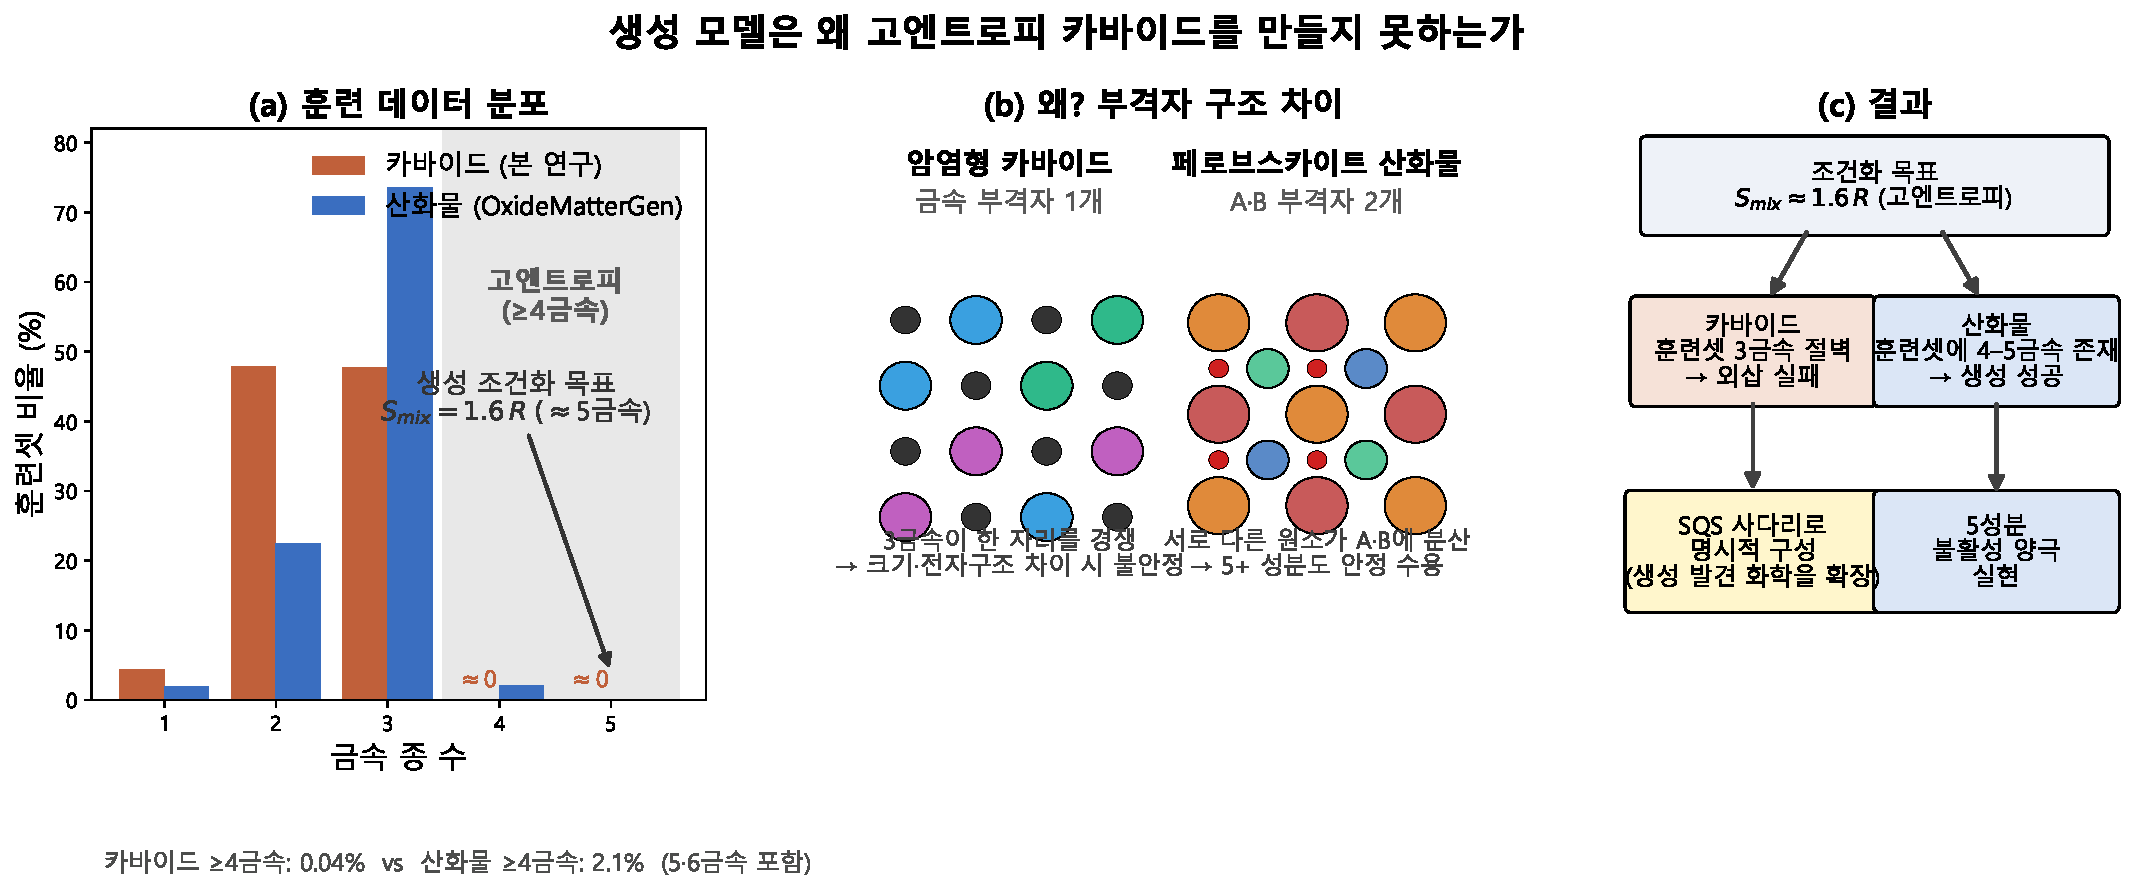
\includegraphics[width=\textwidth]{fig_gen_entropy_limit.pdf}
\caption{생성 모델이 고엔트로피 카바이드를 만들지 못하는 이유와 SQS 사다리의 역할. (a) 훈련셋 금속 종
수 분포(실측): 카바이드(주황)는 3금속에서 절벽($\ge\!4$금속 $0.04\%$)인 반면 산화물(파랑, OxideMatterGen)은
4--6금속이 존재($2.1\%$); 조건화 목표 $S_{\mathrm{mix}}\!=\!1.6\,R$는 카바이드 분포 밖의 외삽이다.
(b) 근본 원인: 암염형 카바이드는 금속 부격자 1개(다금속이 한 자리를 경쟁 → 불안정)인 반면 페로브스카이트
산화물은 A·B 2개 부격자(원소 분산 수용 → 5+ 성분 안정). (c) 결과: 카바이드는 생성 외삽 실패 → SQS
사다리로 명시적 구성; 산화물은 생성으로 5성분 실현.}
\label{fig:genlimit}
\end{figure}

\section{다중탄소 생성물과 다중 자리 탠덤 가설}
\label{sec:tandem}
본 연구의 계산 설계는 CO$_2\!\to\!$CO(2전자)와 HER 억제만을 겨냥하였으나, 예비 전기분해의
\textsuperscript{1}H NMR은 \emph{에탄올} 생성을 보였다(\ref{ch:experiment}장; 정량은 진행 중).
에탄올은 12전자·다중탄소(C\textsubscript{2+}) 생성물로 \emph{C--C 짝지음}을 요구하므로, 이는
설계 목표를 넘어서는 관찰이며 정직한 해석이 필요하다.

\paragraph{단일 자리 관점의 긴장.} 언뜻 이는 설계와 상충하는 듯하다: 최적화한 활성점은
$\dGCO\!\approx\!0$(약결합·방출)인데, 이는 \emph{단일 자리} 기준으로는 오히려 C--C 짝지음에
불리하다 --- 짝지음이 일어나기 전에 CO가 표면을 떠나기 때문이다. 즉 우리가 최적화한 바로 그 자리는
CO \emph{공급원}이지 짝지음 자리가 아니다.

\paragraph{다중 자리 탠덤 가설.} 이 긴장은 \emph{고엔트로피} 표면의 본질---자리 다양성---로 해소된다.
스크리닝은 각 조성의 \emph{최적} 자리($\dGCO\!\approx\!0$)로 순위를 매겼지만, 등몰 다금속 암염
표면은 넓은 $\dGCO$ 분포를 가지며 더 강하게 CO를 붙잡는 자리도 존재한다. 이 강결합 자리들이 CO를
체류시켜 인접 CO와 짝지어 C\textsubscript{2+}로 진행시키는 반면, 약결합 자리는 CO$_2\!\to\!$CO
공급을 담당한다. 따라서 \emph{한 물질이 CO 생성 자리와 C--C 짝지음 자리를 함께 갖는 탠덤 촉매}로
작동할 수 있으며, 관측된 에탄올은 이 창발적 다중 자리 효과로 해석된다. 나아가 H 반발(A2, $\dGH>0$)은
CO뿐 아니라 \emph{모든} CO\textsubscript{2}RR 생성물에 유리하다 --- HER로의 전류 손실과 $*$H 피독을
함께 억제하므로 C\textsubscript{2+} 선택성에도 기여한다.

\paragraph{분기 판정: 어느 심화 경로가 유리한가(계산).} 이 가설을 부분적으로 시험하기 위해, 세 후보
(100) 표면에서 $*$CO의 세 운명 --- CO 방출, C1 심화($*$CHO), C2 짝지음($*$OCCO) --- 의 첫 중간체를
UMA로 계산하였다(흡착종 $*$CHO/$*$OCCO를 파이프라인에 추가). C--C 짝지음($*$OCCO)은 대부분 자리에서
두 CO로 \emph{해리}되나, 물리적으로 짝지은 자리(C--C$\approx$1.5~\AA)가 세 후보 모두 존재하고 그 흡착
자유에너지가 \emph{음}($\Delta G_{*\mathrm{OCCO}}=-0.56\!\sim\!-1.17$~eV, 짝지음 자리 기준)이어서,
\textbf{표면이 CO--CO 짝지음을 안정화}함을 보인다. 반면 C1 심화($*$CHO)는 대체로 \emph{흡열}
($\sim\!+0.8$~eV)이다. 즉 계산은 \textbf{C1(메탄올/메탄)보다 C2(에탄올) 경로가 유리}함을 시사하여,
실험의 에탄올 관찰과 정성적으로 일치한다(그림~\ref{fig:cheher}a에 개념 표시).

\paragraph{한계와 향후 과제.} 위 분기 판정은 \emph{반증 가능}한 부분 검증이나 여러 유의점이 있다:
(i) $*$OCCO 짝지음 \emph{첫 중간체}만 계산했을 뿐 \emph{전체} 에탄올 경로(후속 양성자--전자 전달)와
짝지음 \emph{전이상태·반응 장벽}은 미계산이며, 대부분 자리가 해리로 가므로(짝지음은 특정 자리에서만)
C--C 짝지음은 UMA(학습분포 밖) 수준의 \emph{정성} 신호로 DFT 검증이 필요하다($*$OCCO/$*$CHO의 영점진동
보정도 근사값); (ii) 에탄올은 최적 자리가 아니라
\emph{자리 분포}에서 비롯하므로, 활성 순위와 직접 연결되지 않는다; (iii) 에탄올 대 CO 분배(패러데이
효율)는 미정량이다. 향후 과제는 자리 분포에 걸친 CO--CO 짝지음 에너지론을 제일원리로 계산하고,
\emph{짝지음 디스크립터를 조건화 속성으로 추가}하여 C\textsubscript{2+} 선택성을 능동적으로 설계하는
것이다. 요컨대 본 논문은 CO 생성·HER 억제라는 \emph{필요조건}을 설계·검증하였고, 에탄올은 그 위에서
고엔트로피 표면이 보인 고무적 실험 결과로서 C\textsubscript{2+}로의 확장 경로를 제시한다.

\section{한계와 정직한 유의점}
몇 가지 유의점을 명시해야 한다. (i) 경희토류(La, Ce, Pr, Y)는 선택한 디스크립터상 경제적으로 ``저렴''
하지만, 희토류 카바이드는 이례적인 CO\textsubscript{2}RR 촉매이며 친산소성이고 공기/수분에 민감할 수
있다. 실험적 견고성은 계획된 안정성 시험이 직접 다루는 미해결 문제이다. (ii) MLIP 표면 스크리닝은 기준
오차를 상쇄하도록 보정되었지만, 학습 분포의 대부분 바깥에 있는 희토류 카바이드 표면을 평가한다. 특히
강하게 결합한 *COOH 에너지는 정성적으로 읽어야 하며, 활성 순위는 더 견고한 $\dGCO$ 디스크립터에 의존한다.
(iii) Stage A--B에 사용된 조성 대리지표는 정량 예측이 아니라 거친 필터링을 위한 문헌 기반 추정치이다.
(iv) DFT는 희토류 $4f$ 전자를 고정된 3가 코어로 취급한다. 이는 이들 금속성 카바이드에 적절하지만,
$f$-상태에 민감한 물성에는 $4f$-원자가 또는 DFT$+U$ 처리가 필요하다. (v) 현재 DFT는 \emph{벌크} 안정성과
금속성을 검증한다. DFT에서의 명시적 무질서 \emph{표면} 자유에너지(Stage A$'$의 SQS 슈퍼셀 위)는 여기서
보고한 MLIP 수준 표면 스크리닝을 넘어서는 자연스러운 다음 전산 단계이다. 이러한 한계는
\ref{ch:experiment}장의 실험 캠페인을 약화시키기보다 동기를 부여하며, 실험이 예측의 심판자이다.

\section{전망}
캠페인 B의 Ti 기반 후보 확인을 넘어, 두 캠페인 대비는 \emph{제약을 생성 단계에 넣는 것}의 가치를 보였다:
캠페인 B에서 생성기를 저-VEC로 재조준하자 모형 자체가 H-반발 후보를 산출하였고, 이는 발견이 후처리
스크린이 아니라 조건화에서 나올 수 있음을 시사한다. 파이프라인은 실험 및 상위 수준 DFT 데이터가 조성
대리지표와 MLIP를 재보정하여 연속 세대를 정밀화하는 능동학습(active-learning) 루프를 지원한다. 동일한
조건부 생성기는 조건화 디스크립터를 변경함으로써 CO\textsubscript{2}-to-폼산 또는 다중 탄소 생성물로
재조준될 수 있다.

% =====================================================================
\chapter{결론}
\label{ch:conclusion}

본 논문은 우수한 CO\textsubscript{2}RR 카바이드 촉매의 네 설계 공리(활성·선택성·제조 가능성·경제성)를
물성 조건부 확산 모델에 내재화하고, \emph{하나의 파이프라인을 두 제약 집합으로 구동}하여 이들을
기계학습 퍼텐셜과 제일원리 DFT의 깔때기로 검증하였다. \emph{캠페인 A}(활성-우선 기준선)는 1024개
생성 구조에서 6개의 백금족-무함유 고엔트로피 카바이드를 도출하고, 표면 자유에너지·$d$-밴드·볼록 껍질과
같은-면 표면 Pourbaix로 특성화하였다(작동 전위에서 산화가 아니라 반응 중간체 $*$COOH가 정지상태). 그러나
이 후보군은 \emph{제조 가능성 관문}에서 탈락한다 --- 금속열환원--\emph{산-침출} 합성의 필수 침출 단계에서
희토류가 용해되어 제조 불가이다. 이는 실패가 아니라 통제된 대조로서, \emph{제약 없는 활성 탐색이 제조
불가능한 화학으로 수렴함}을 보이고 제조 가능성을 생성 제약으로 승격시켜야 함을 입증한다.

\emph{캠페인 B}는 네 공리를 모두 부과한다: 탐색 공간을 산-침출 안정 4/5/6족 전이금속으로 한정하고
(희토류·백금족과 더불어, 생성 모형의 발견 기여를 담보하기 위해 알려진 CO$_2$RR 금속 Cu/Ag/Au/Zn도
배제), UMA 계산 표면 라벨로 조건화하며, HER 경쟁을 명시적으로 다루어 --- 강한 H 흡착은 CO$_2$ 사이트를
덮는 \emph{피독}이므로 --- CO 발생($|\dGCO|<0.3$)과 \emph{H 반발}($\dGH>0$)을 같은 면에서 동시 요구하는
\emph{이중 활성점} 기준을 적용한다. 희토류는 제조상 배제되고 활성점 설계상으로도 \emph{불필요}한데, 이중
거동이 전이금속의 원자가전자농도(VEC) 효과이기 때문이다(두 근거는 독립). 그 결과 \textbf{3종의 Ti 기반
3금속 암염형 카바이드(hec3-MoTiZr/CrTiV/CrTiZr, (100))가 DFT 이중목표를 통과}하였고, H 피독이 지배적
실패 양식이며 낮은 VEC가 H 반발과 CO 발생을 함께 조율하는 물리적 레버임을 확인하였다. 대표 후보
hec3-MoTiZr의 완전 이온 이완은 \emph{선택성을 확증}하되($\dGH\!=\!+0.57$~eV, 오히려 강화;
$\dGCO\!=\!+0.18$~eV) \emph{한계 전위를 $U_L\!=\!-0.40$~V로 정정}하여, 단일점이 $*$COOH 장벽을
과소평가했음을 보였다. 마지막으로 생성기를 저-VEC로 재조준하자 \emph{생성 모형 자체가} H-반발·CO-발생
승자를 산출하여, 발견이 후처리 스크린이 아니라 조건부 생성에서 나올 수 있음을 입증하였다.

이 예측을 시험하기 위해 합성, 전기화학 CO\textsubscript{2}RR, 온라인 가스 분석, \textsuperscript{1}H NMR,
in-situ FT-IR로 이루어진 실험 검증 프로그램을 설계하였다(\ref{ch:experiment}장). 더 넓은 기여는 촉매
발견에서 경제성·\emph{합성 가능성}·\emph{HER 선택성}을 모두 \emph{생성적} 설계 목표로 삼을 수 있으며,
합성 현실(산-침출)이 원소 팔레트를 규정하고 물리(수소 피독)가 조건화 레버(VEC)를 규정함을 재사용 가능하게
보인 것이다.

% =====================================================================
\begin{thebibliography}{99}
\setlength{\itemsep}{2pt}

\bibitem{zeni2025} C.~Zeni, R.~Pinsler, D.~Z\"ugner, A.~Fowler, M.~Horton, X.~Fu, Z.~Wang,
A.~Shysheya, J.~Crabb\'e, S.~Shysheya, \emph{et al.},
``A generative model for inorganic materials design,''
\emph{Nature} \textbf{639}, 624--632 (2025). doi:10.1038/s41586-025-08628-5.

\bibitem{uma2025} B.~M.~Wood, M.~Dzamba, X.~Fu, M.~Gao, M.~Shuaibi, L.~Barroso-Luque,
K.~Abdelmaqsoud, V.~Gharakhanyan, J.~R.~Kitchin, \emph{et al.},
``UMA: A Family of Universal Models for Atoms,'' arXiv:2506.23971 (2025).

\bibitem{chanussot2021} L.~Chanussot, A.~Das, S.~Goyal, T.~Lavril, M.~Shuaibi, M.~Riviere,
K.~Tran, J.~Heras-Domingo, C.~Ho, W.~Hu, \emph{et al.},
``Open Catalyst 2020 (OC20) Dataset and Community Challenges,''
\emph{ACS Catal.} \textbf{11}, 6059--6072 (2021). doi:10.1021/acscatal.0c04525.

\bibitem{giannozzi2009} P.~Giannozzi, S.~Baroni, N.~Bonini, M.~Calandra, R.~Car, C.~Cavazzoni,
D.~Ceresoli, G.~L.~Chiarotti, M.~Cococcioni, I.~Dabo, \emph{et al.},
``QUANTUM ESPRESSO: a modular and open-source software project for quantum simulations of
materials,'' \emph{J. Phys.: Condens. Matter} \textbf{21}, 395502 (2009).
doi:10.1088/0953-8984/21/39/395502.

\bibitem{prandini2018} G.~Prandini, A.~Marrazzo, I.~E.~Castelli, N.~Mounet, N.~Marzari,
``Precision and efficiency in solid-state pseudopotential calculations,''
\emph{npj Comput. Mater.} \textbf{4}, 72 (2018). doi:10.1038/s41524-018-0127-2.

\bibitem{pbe1996} J.~P.~Perdew, K.~Burke, M.~Ernzerhof,
``Generalized Gradient Approximation Made Simple,''
\emph{Phys. Rev. Lett.} \textbf{77}, 3865--3868 (1996). doi:10.1103/PhysRevLett.77.3865.

\bibitem{norskov2004} J.~K.~N\o{}rskov, J.~Rossmeisl, A.~Logadottir, L.~Lindqvist,
J.~R.~Kitchin, T.~Bligaard, H.~J\'onsson,
``Origin of the Overpotential for Oxygen Reduction at a Fuel-Cell Cathode,''
\emph{J. Phys. Chem. B} \textbf{108}, 17886--17892 (2004). doi:10.1021/jp047349j.

\bibitem{nitopi2019} S.~Nitopi, E.~Bertheussen, S.~B.~Scott, X.~Liu, A.~K.~Engstfeld, S.~Horch,
B.~Seger, I.~E.~L.~Stephens, K.~Chan, C.~Hahn, J.~K.~N\o{}rskov, T.~F.~Jaramillo, I.~Chorkendorff,
``Progress and Perspectives of Electrochemical CO\textsubscript{2} Reduction on Copper in Aqueous
Electrolyte,'' \emph{Chem. Rev.} \textbf{119}, 7610--7672 (2019).
doi:10.1021/acs.chemrev.8b00705.

\bibitem{hori2008} Y.~Hori, ``Electrochemical CO\textsubscript{2} Reduction on Metal Electrodes,''
in \emph{Modern Aspects of Electrochemistry}, vol.~42, eds.\ C.~G.~Vayenas \emph{et al.},
Springer, New York, pp.~89--189 (2008). doi:10.1007/978-0-387-49489-0\_3.

\bibitem{batchelor2019} T.~A.~A.~Batchelor, J.~K.~Pedersen, S.~H.~Winther, I.~E.~Castelli,
K.~W.~Jacobsen, J.~Rossmeisl,
``High-Entropy Alloys as a Discovery Platform for Electrocatalysis,''
\emph{Joule} \textbf{3}, 834--845 (2019). doi:10.1016/j.joule.2018.12.015.

\bibitem{nellaiappan2020} S.~Nellaiappan, N.~K.~Katiyar, R.~Kumar, A.~Parui, K.~D.~Malviya,
K.~G.~Pradeep, A.~K.~Singh, S.~Sharma, C.~S.~Tiwary, K.~Biswas,
``High-Entropy Alloys as Catalysts for the CO\textsubscript{2} and CO Reduction Reactions:
Experimental Realization,'' \emph{ACS Catal.} \textbf{10}, 3658--3663 (2020).
doi:10.1021/acscatal.9b04302.

\bibitem{levy1973} R.~B.~Levy, M.~Boudart,
``Platinum-Like Behavior of Tungsten Carbide in Surface Catalysis,''
\emph{Science} \textbf{181}, 547--549 (1973). doi:10.1126/science.181.4099.547.

\bibitem{porosoff2014} M.~D.~Porosoff, X.~Yang, J.~A.~Boscoboinik, J.~G.~Chen,
``Molybdenum Carbide as Alternative Catalysts to Precious Metals for Highly Selective Reduction of
CO\textsubscript{2} to CO,'' \emph{Angew. Chem. Int. Ed.} \textbf{53}, 6705--6709 (2014).
doi:10.1002/anie.201404109.

\bibitem{sarker2018} P.~Sarker, T.~Harrington, C.~Toher, C.~Oses, M.~Samiee, J.-P.~Maria,
D.~W.~Brenner, K.~S.~Vecchio, S.~Curtarolo,
``High-entropy high-hardness metal carbides discovered by entropy descriptors,''
\emph{Nat. Commun.} \textbf{9}, 4980 (2018). doi:10.1038/s41467-018-07160-7.

\bibitem{zunger1990} A.~Zunger, S.-H.~Wei, L.~G.~Ferreira, J.~E.~Bernard,
``Special quasirandom structures,'' \emph{Phys. Rev. Lett.} \textbf{65}, 353--356 (1990).
doi:10.1103/PhysRevLett.65.353.

\bibitem{pymatgen2013} S.~P.~Ong, W.~D.~Richards, A.~Jain, G.~Hautier, M.~Kocher, S.~Cholia,
D.~Gunter, V.~L.~Chevrier, K.~A.~Persson, G.~Ceder,
``Python Materials Genomics (pymatgen): A robust, open-source python library for materials
analysis,'' \emph{Comput. Mater. Sci.} \textbf{68}, 314--319 (2013).
doi:10.1016/j.commatsci.2012.10.028.

\bibitem{ase2017} A.~Hjorth Larsen, J.~J.~Mortensen, J.~Blomqvist, I.~E.~Castelli, R.~Christensen,
M.~Du\l{}ak, J.~Friis, M.~N.~Groves, B.~Hammer, C.~Hargus, \emph{et al.},
``The atomic simulation environment---a Python library for working with atoms,''
\emph{J. Phys.: Condens. Matter} \textbf{29}, 273002 (2017). doi:10.1088/1361-648X/aa680e.

\end{thebibliography}

\end{document}
